% Copyright (C) 2014-2016 by Thomas Auzinger <thomas@auzinger.name>

\documentclass[draft,final]{vutinfth} % Remove option 'final' to obtain debug information.

% Load packages to allow in- and output of non-ASCII characters.
\usepackage{lmodern}        % Use an extension of the original Computer Modern font to minimize the use of bitmapped letters.
\usepackage[T1]{fontenc}    % Determines font encoding of the output. Font packages have to be included before this line.
\usepackage[utf8]{inputenc} % Determines encoding of the input. All input files have to use UTF8 encoding.

% Extended LaTeX functionality is enables by including packages with \usepackage{...}.
\usepackage{amsmath}    % Extended typesetting of mathematical expression.
\usepackage{amssymb}    % Provides a multitude of mathematical symbols.
\usepackage{mathtools}  % Further extensions of mathematical typesetting.
\usepackage{microtype}  % Small-scale typographic enhancements.
\usepackage[inline]{enumitem} % User control over the layout of lists (itemize, enumerate, description).
\usepackage{multirow}   % Allows table elements to span several rows.
\usepackage{booktabs}   % Improves the typesettings of tables.
\usepackage{subcaption} % Allows the use of subfigures and enables their referencing.
\usepackage[ruled,linesnumbered,algochapter]{algorithm2e} % Enables the writing of pseudo code.
\usepackage[usenames,dvipsnames,table]{xcolor} % Allows the definition and use of colors. This package has to be included before tikz.
\usepackage{nag}       % Issues warnings when best practices in writing LaTeX documents are violated.
\usepackage{todonotes} % Provides tooltip-like todo notes.
\usepackage{hyperref}  % Enables cross linking in the electronic document version. This package has to be included second to last.
\usepackage[acronym,toc]{glossaries} % Enables the generation of glossaries and lists fo acronyms. This package has to be included last.

% Define convenience functions to use the author name and the thesis title in the PDF document properties.
\newcommand{\authorname}{Bernhard Rainer} % The author name without titles.
\newcommand{\thesistitle}{Interactive Shape Detection in Out-Of-Core Point-Clouds for assisted User
	Interactions} % The title of the thesis. The English version should be used, if it exists.

% Set PDF document properties
\hypersetup{
    pdfpagelayout   = TwoPageRight,           % How the document is shown in PDF viewers (optional).
    linkbordercolor = {Melon},                % The color of the borders of boxes around crosslinks (optional).
    pdfauthor       = {\authorname},          % The author's name in the document properties (optional).
    pdftitle        = {\thesistitle},         % The document's title in the document properties (optional).
    pdfsubject      = {Subject},              % The document's subject in the document properties (optional).
    pdfkeywords     = {a, list, of, keywords} % The document's keywords in the document properties (optional).
}

\setpnumwidth{2.5em}        % Avoid overfull hboxes in the table of contents (see memoir manual).
\setsecnumdepth{subsection} % Enumerate subsections.

\nonzeroparskip             % Create space between paragraphs (optional).
\setlength{\parindent}{0pt} % Remove paragraph identation (optional).

\makeindex      % Use an optional index.
\makeglossaries % Use an optional glossary.
%\glstocfalse   % Remove the glossaries from the table of contents.

% Set persons with 4 arguments:
%  {title before name}{name}{title after name}{gender}
%  where both titles are optional (i.e. can be given as empty brackets {}).
\setauthor{}{\authorname}{BSc.}{male}
\setadvisor{Pretitle}{Michael Wimmer}{Posttitle}{male}

% For bachelor and master theses:
%\setfirstassistant{Pretitle}{Forename Surname}{Posttitle}{male}
%\setsecondassistant{Pretitle}{Forename Surname}{Posttitle}{male}
%\setthirdassistant{Pretitle}{Forename Surname}{Posttitle}{male}

% For dissertations:
\setfirstreviewer{Pretitle}{Forename Surname}{Posttitle}{male}
\setsecondreviewer{Pretitle}{Forename Surname}{Posttitle}{male}

% For dissertations at the PhD School and optionally for dissertations:
\setsecondadvisor{Pretitle}{Forename Surname}{Posttitle}{male} % Comment to remove.

% Required data.
\setaddress{Heigerleinstraße 53 8, 1170 Wien}
\setregnumber{0828592}
\setdate{1}{03}{2017} % Set date with 3 arguments: {day}{month}{year}.
\settitle{\thesistitle}{\thesistitle} % Sets English and German version of the title (both can be English or German).
%\setsubtitle{Optional Subtitle of the Thesis}{Optionaler Untertitel der Arbeit} % Sets English and German version of the subtitle (both can be English or German).

% Select the thesis type: bachelor / master / doctor / phd-school.
% Bachelor:
%\setthesis{bachelor}
%
% Master:
\setthesis{master}
\setmasterdegree{dipl.} % dipl. / rer.nat. / rer.soc.oec. / master
%
% Doctor:
%\setthesis{doctor}
%\setdoctordegree{rer.soc.oec.}% rer.nat. / techn. / rer.soc.oec.
%
% Doctor at the PhD School
%\setthesis{phd-school} % Deactivate non-English title pages (see below)

% For bachelor and master:
\setcurriculum{Visual Computing}{Visual Computing} % Sets the English and German name of the curriculum.

% For dissertations at the PhD School:
\setfirstreviewerdata{Affiliation, Country}
\setsecondreviewerdata{Affiliation, Country}


\begin{document}

\frontmatter % Switches to roman numbering.
% The structure of the thesis has to conform to
%  http://www.informatik.tuwien.ac.at/dekanat

\addtitlepage{naustrian} % German title page (not for dissertations at the PhD School).
\addtitlepage{english} % English title page.
\addstatementpage

\begin{danksagung*}
\todo{Ihr Text hier.}
\end{danksagung*}

\begin{acknowledgements*}
\todo{Enter your text here.}
\end{acknowledgements*}

\begin{kurzfassung}
\todo{Ihr Text hier.}
\end{kurzfassung}

\begin{abstract}
\todo{Enter your text here.}
\end{abstract}

% Select the language of the thesis, e.g., english or naustrian.
\selectlanguage{english}

% Add a table of contents (toc).
\tableofcontents % Starred version, i.e., \tableofcontents*, removes the self-entry.

% Switch to arabic numbering and start the enumeration of chapters in the table of content.
\mainmatter


\chapter{Introduction}

\section{Motivation}

In recent years, multiple acquisition devices and methods of point clouds from real objects have emerged, such as laser scanners, LIDAR, Microsoft Kinect, or photogrammetric reconstructions. The fields of applications for point clouds include, but are not limited to, documenting geomorphological erosion, monitoring urban and agricultural developments, mapping archeological sites, and generating assets for the entertainment industry. The acquisition techniques produce highly detailed point clouds that contain several millions of points. This enormous data resolution presents several challenges to both the system and the user. 

\par

% Challenges to the system
The size of point-cloud datasets has increased at such a rapid rate that they are now simply too large to fit into system memory, let alone graphics card memory. Therefore, new solutions for out-of-core representations have emerged. In most of these solutions, the point cloud data is cached in one or more structured files on the hard drive and can therefore not be accessed directly. Based on a culling heuristic, chunks of point-cloud data are loaded into memory as needed. This continuous swapping of data yields the disk speed as a potential bottleneck when it comes to performance. However, it also introduces the benefit of only storing chunks of data in memory that are of immediate interest to the user. 

\par

% Challenges to the user
Point-cloud datasets commonly lack structure and contain a lot of unneeded data. Thus, additional processing is required to enrich the data set with semantic information. To improve data quality, additional postprocessing steps must be performed by the user manually, such as removing imperfect regions, extracting regions of interest. However, achieving this task by using classic two-dimensional interaction metaphors can be tedious and cumbersome as the system cannot predict the desired boundaries of the third dimension of the interaction. Without the use of more semantic information, such as the geometric shape of the region of interest, multiple view changes might be necessary to only select desired regions from the three-dimensional scene. 

\par

% Lack of semantic information
A way of introducing semantic information into unstructured point-cloud data is shape detection. The objective is to find regions in point clouds with similar characteristics, such as local curvature and neighborhoods, to help the user understand local and global structures. Current solutions, as presented by Schnabel et al. \cite{schnabel-2007-efficient, schnabel-2007-ransac}, can already produce a precise segmentation of point clouds. The complexity of these algorithms increases with the size of the point cloud, making the computation for billions of points infeasible in real time. However, when looking at raw numbers, the approach delivers promising results in a fraction of a second for point clouds of smaller size (<12,000 points).

\par

This thesis proposes a user-controlled technique for shape detection in small local regions of point clouds. This approach can to deliver semantic information on the local geometry in interactive time. This information is used to improve ordinary two-dimensional interaction metaphors by limiting the set of points available for interaction to those that belong to the selected shape (i.e. closely follow the curvature of the shape). 


\section{Problem Definition}

Modern point clouds can contain millions of points with it's size often exceeding several gigabytes. Usually, consumer PCs do not have the memory capacity to hold the entire point cloud in system memory or video memory. Efficient out-of-core solutions for point clouds are discussed in numerous publications, Scheibelbauer \cite{scheiblauer-thesis}, Elseberg et al. \cite{elseberg2013one} or the Point Cloud Library \cite{rusu20113d}, to only name a few. However, a custom solution is needed that stores point clouds enriched with semantic information.

\par

In scans of urban environments, many structures can be represented in a more memory-efficient way. Points that follow a wall can often be compressed to few triangles. Pillars often share similarities with cylinders. Detecting such shapes is an immense task that scales with the number of points and fails to be executed in real time. When exploring a point cloud, immediate feedback of local geometry is useful, since it introduces additional information to the user. This task cannot be achieved without substantial postprocessing of the point cloud. 

\par

Common two-dimensional interaction metaphors (e.g. mouse) are useful tools when selecting or picking regions from a two-dimensional context. When porting these techniques to 3D, the third dimension (i.e. depth) must be guessed or controlled separately. A region of interest usually is a set of points that are spatial neighboring and create a structural element in the point cloud. Ideally, the selection of such a region is performed by defining a minimal enclosing volume that contains all points. Achieving this selection by using 2D-interaction metaphors only is challenging, as the techniques do not know the desired depth boundaries of the selection region. Therefore, interactions across multiple views are needed to achieve this selection. Methods that use 3D information, such as the volumetric brush presented by Weyrich et al. \cite{weyrich2004post}, can ease selection tasks. By consulting the depth buffer each frame, the brush follows the curvature of the furthermost geometry. However, by reading pixels from the GPU, the rendering process is stalled. This technique reacts to occlusion such that the brush follows the geometry depicted in the depth buffer, rather then the desired structure. Thus, view changes are still required.


\section{Contributions}

The main contribution of this diploma thesis is the implementation of a semi-automated procedure to detect shapes in multiple levels of detail in point clouds. Instead of performing shape detection on the entire point cloud at once, our approach lets the user control the region in which shapes should be detected. By reducing those regions to a suitable size, a well-known shape detection algorithm can return meaningful results in interactive time, such that the user is presented with immediate feedback on the local geometry of the selected region. 

\par

Contribution dynamic epsilon for shape detection based on the regions density. 

\par

Shapes are detected in multiple levels of detail in the point cloud. A clustering algorithm finds shapes in different different regions and levels of detail, based on a similarity heuristic, and creates a larger connected cluster of shapes. This cluster is used to present geometric information on a larger scale to the user, rather than each shape separately. 

\par

This thesis proposes several improvements to commonly known user interactions. \textit{Point picking} and \textit{region selection} are improved by consulting the local geometry of the point cloud to assist the user. By using a shape as support, the interaction dimensions are reduced to the parameter space of the shapes, allowing the user to exclude unwanted points from interactions easily. 

\par

Additionally, a novel interaction technique is introduced that allows the user to increment the level of detail locally along a shape. This helps the user to explore the structure of the point cloud in more detail. 


\section{Structure of the Work}

Chapter \ref{chap:related_work} covers the related work for this thesis, including point-cloud rendering and out-of-core representations, shape detection, and segmentation and advanced user interactions on point clouds. Chapter \ref{chap:octree} describes the octree used for the out-of-core representation of the point cloud, as well as some metrics that further describe the content of an octree node. Chapter \ref{chap:shapeDetection} describes the algorithms used to detect primitive shapes in a point cloud and proposes a technique to cluster similar shapes into one coherent shape cluster for user interactions. Chapter \ref{chap:systemDesign} discusses the application's features, including the user-controlled shape detection and assisted interactions that utilize the detected shapes as support shape. Chapter \ref{chap:implementation} focuses on implementation details in a functional context. Results of the application are presented in Chapter \ref{chap:results}. Chapter \ref{chap:conclusion} concludes this thesis with a reflection on the application and an outlook on future work. 
 
\chapter {Related Work}
\label{chap:related_work}

This chapter gives an overview over work that is related to this thesis. Section \ref{sec:related_work_point_clouds} presents related work on storing and rendering out-of-core point clouds, Section \ref{sec:related_work_shape detection} shows ways on to detected shapes in point clouds. Related work on interactions is presented in Section \ref{sec:related_work_interactions}. 

\section {Out-of-Core Point-Clouds}
\todo{}
\cite{gobbetti2004layered}
\cite{wimmer2006instant}
\cite{wand2007interactive}
\cite{SCHUETZ-2016-POT}
\chapter{Shape Detection}
\label{chap:shapeDetection}


\section{Overview}

This thesis utilizes shape detection to automatically detect primitive shapes for small parts of the point cloud at a time. It is designed in such a way that the user receives immediate feedback of local geometry for the region under the mouse cursor. The approach utilizes an automated shape detection algorithm that is capable of detecting different types of primitive shapes. This algorithm is designed to find shapes in point clouds that consist of several million points within minutes. However, when looking at the performance for smaller samples, results can be achieved at interactive time rates. Section \ref{sec:schnabel} describes the shape detection algorithm in detail. 
\\

Before using the detected shapes for rendering or interactions, the shapes must be postprocesssed. Since some of the shapes are of infinite size, they need to be refitted to encapsulate the corresponding support points and create a minimal boundary. Section \ref{sec:Refitting} describes this task. 
\\

Section \ref{sec:shapeMatching} proposes a set of heuristics to determine if detected primitive shapes originate from the same geometric structure. Section \ref{sec:shapeClustering} explains the usage of this heuristics in order to create larger, homogeneous cluster of shapes, used for interactions. 


\section{Efficient RANSAC for Point-Cloud Shape Detection}
\label{sec:schnabel}

The section gives a brief overview over the algorithm used to detect primitive shapes. 
Schnabel et al. \cite{schnabel-2007-efficient} propose an automated way to detect simple primitive shapes in unstructured point clouds. The point cloud is decomposed into a set of shapes and a set of unused points. The algorithm supports detection of planes, spheres, cylinders, cones, and tori. 

\textbf{RAN}dom \textbf{SA}mpling \textbf{C}onsens (RANSAC) was first discussed by Fischler and Bolles \cite{fischler1981random} as a paradigm for model fitting for image analysis and automated cartography. However, this approach can be generalized for points with an origin other than images. The shape detection utilizes RANSAC to repeatedly take a minimal set of points to build a primitive shape $\Psi$ and checks if the points in the region roughly follow the curvature of the shape. 

\subsection{Minimal sets}

A minimal set describes the set of points that are needed to construct a candidate shape. 
For each type of shape, the following rule applies: A shape is only considered as candidate shape if all points from the minimal set are within a distance $\epsilon$ to the shape and the normal does not deviate from the shape's normal by more than an angle $\alpha$. 

\begin{itemize}
    \item \textbf{Plane}: A plane is constructed from three points $p_0, p_1, p_2$ whose normals do deviate from the plane's normal less than the angle $\alpha$. 
    
    \item \textbf{Sphere}: A sphere is fully defined by two points $p_0, p_1$ with corresponding normal vectors $n_0, n_1$. The center $c$ of the sphere is defined by the midpoint shortest line segment between the parametric lines $p_0 + tn_0$ and $p_1 + sn_1$. The radius is constructed by averaging the distance of $p_0$ and $p1$ to $c$.

    \item \textbf{Cylinder}:
    In order to create a cylinder, a minimal set of two points  $p_0, p_1$ with corresponding normal vectors $n_0, n_1$ is used. The direction $d$ of the axis is established by $d = n_0 \times n_1$. The origin $c$ of the cylinder is created by projecting the parametric lines $p_0 + tn_0$ and $p_1 + sn_1$ onto the plane $d \cdot x = 0$ and taking their intersection as origin $c$. The radius is the shortest distance between $p_0$ and the axis $c + ud$
    
    \item \textbf{Cone}:
    For simplicity, the minimal set for a cone consists of three points $p_0, p_1, p_2$, rather than two. For each point-normal pair, a plane is created. The intersection of the three planes defines the apex $c$. To describe the direction of the axis a plane is constructed from the points \{$c +  \frac{p_0 - c}{||p_0 - c||}$, $c +  \frac{p_1 - c}{||p_1 - c||}$, $c +  \frac{p_2 - c}{||p_2 - c||}$\}. The normal of this plane is the direction $d$ of the cone axis. The opening angle is given as $\omega = \frac{\sum_{i}^{max} (p_i - c)\cdot d}{3}$
    
    \item \textbf{Torus}:
    A minimal set of four points with normals is used, one more than theoretically necessary, However, this eases the computation.
    Two possible rotational axis are found by intersecting the four point-normal lines $p_i +  \lambda n_i$\cite{marshall2001robust}. For each axis, a full torus is estimated, and the torus is chosen that causes the smaller error in respect to the four points. The minor radius is found by projecting the points onto a plane that rotates around the axis. A circle is constructed using three points, whose radius is the minor radius of the torus. The major radius is given as the distance from the circle center to the axis. 


\end{itemize} 

\subsection{Score function}
\label{sec:scorefun}
To only use points that roughly follow the curvature of a candidate shape, only points within a distance $\epsilon$ are taken into account. Furthermore, each point must fulfill a score function to be considered a support point of the shape $\Psi$. 
The score function for each point consists of the following: 
\begin{itemize}
    \item The distance between the point and the shape must be smaller than $\epsilon$.
    \item The normal of the point must not deviate from the normal of the shape more than a given angle $\alpha$.
    \item Among all points that fulfill the previous two conditions, only the subset of points, which creates the largest connected component embedded in the shape,  is considered.
\end{itemize}

All points that are within a distance $\epsilon$ are taken into account. However, only those whose normals do not deviate from the normal of the shape more than a given angle $\alpha$ are considered support points. Additionally, the number of support points must exceed a threshold value $n$ for this shape to be valid. 


\subsection{Performance}

\begin{table}
    \centering
    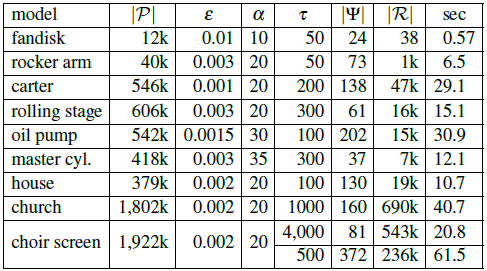
\includegraphics[width=0.7\textwidth]{Shape_Detection/schnabel-performance.png}
    \caption[Original statistics of the shape detection algorithm by Schabel et al.]{The original statistics by Schnabel et al. \cite{schnabel-2007-efficient} on processed models. $\epsilon$ is given as ration of maximum bounding box with. Results have been averaged over 5 runs and rounded.}
    \label{table:schnabel_performance}
\end{table}

Table \ref{table:schnabel_performance} describes the statistical results for different models. $|P|$ is the number of points, $\epsilon$ the distance threshold, $\alpha$ the maximum normals deviation, $\tau$ is the minimum number of support points, $\|Psi|$ the number of shapes found, $|R|$ the number of RANSAC iterations. It can be seen that for small a small number of points and weaker constraints the algorithm returns plausible results within a fraction of a second. We utilize this feature the detect shapes in our application for small regions at a time to give immediate feedback to the user. 


\section{Refitting}
\label{sec:Refitting}

Planes, cylinder, and cones are infinite shapes. Therefore, to use those shapes for rendering and interactions, it is necessary to create finite representations for each shape. Each shape comes with the corresponding set of support points that are used to refit the shape. Spheres and Tori are finite by definition. Therefore they do not require refitting. 


\subsection{Refitting planes}

Planes, however, are represented by a point and a vector. All support points are projected onto the plane, thus reducing the fitting problem to two dimensions. The procedure starts by computing the convex hull of the projected points with the help of Andrew's monotone chain 2d convex hull algorithm\cite{andrew1979another}. 
More complex polygons can be computed. However, for this purpose, a quad is sufficient. The quad is obtained by using the minimum-bounding-rectangle algorithm by Freeman\cite{freeman1975determining}. 


\subsection{Refitting cylinder}

A cylinder is defined by a center $p$, direction vector $v$ and a radius $r$. The height of the cylinder is chosen as the maximum distance between two support points on the axis of the cylinder. This is achieved by projecting all points onto the axis $a = p + vt$ of the cylinder, and select the points $p_{min}$, where $t$ is minimum and $p_{max}$, where $t$ is maximum. The distance $d$ between $p_{min}$ and $p_{max}$ is the height of the enclosing cylinder. The cylinder is refitted such that the new center is set to $p' = p_{min}$ and the $d$ is encoded in the length of the new direction vector:$v' = \frac{v}{|v|}d$. The radius stays the same. 


\subsection{Refitting cones}

A cone is defined by its apex $c$, axis direction $v$, and opening angle $\theta$. Similar to the cylinder, all support points are projected onto the axis and the points $p_{min}, p_{max}$, with minimum and maximum $t$, are selected. Since the apex of a cone is fixed, the range cannot be encoded using $c$ and $v$. The range is stored separately. Range checks are performed when rendering or interacting with cones. 


\section{Shape Detection Parameter Selection}
\label{sec:shapeDetectionParameterSelection}

This section briefly discusses the issue of selecting optimal parameters for the shape detection. The $\epsilon$ parameter creates an $\epsilon$-band that follows the curvature of the shape. All points within this $\epsilon$ band are considered to be candidates. The authors propose to use the point cloud's bounding boxes largest dimension times $0.1$ as $\epsilon$. However, using such a static parameter yields problems with extremely sparse regions and regions that are populated very densely. In this thesis, shape detection is performed dynamically on local regions of the point cloud at a time. The local density of an octree node is chosen as $\epsilon$. The density is calculated per octree node by averaging the distance of each point to its nearest neighbor. Thus, nodes that are populated more densely create finer geometry. 

The $\alpha$ parameter is used to determine the deviation between two directions. As the normals are the same at different level-of-detail, this parameter is static. We use an $\alpha$ value of $0.95$. 

The minimum number of support points per shape is set to $250$.
\chapter{Interactions}

Creating new interactions is a key topic for this thesis. This chapter describes the pros and cons of current state-of-the-art two-dimensional interactions and proposes improvements using the detected primitive shapes as interaction support shapes. 

Many proven interaction techniques have emerged over time, such as \textit{Point Picking} or \textit{Region Selection}. 

%% TODO: define pick ray
%% TODO: define candidate global
%% TODO: define point belongs to a shape

\section{Shape Picking}


\section{Point Picking}
\label{sec:picking}
\textit{Point Picking} describes an interaction, where the user is interested in selecting a single point from the scene at a time. A \textit{pick ray} describes a ray originating from the mouse position whose direction is the view direction. The pick radius $r$ denotes the maximum distance of a point to the pick ray in order for the point to be considered a candidate point. Depending on the use case the pick radius $r$ can be depended on the depth value. There are multiple ways of implementing this interaction with varying results. 
\\
\\
The first explored technique is to use a fixed pick radius in world space. The picked point is the point closest to the pick ray in world space. Since the user only interacts with points that are projected onto the nearplane, the projection of the pick radius is smaller for points that lie in the background. Therefore, the distance in pixel between the mouse position and a picked point in the background is smaller than the distance to a picked point in the foreground. While this encourages the picking of points in the foreground, the non-uniform pixel distance introduces inconsistencies. 
\\
\\
A more consistent way of picking a point is to only use the screen space information for each point. The mouse position $p$ in screen space combined with the pick radius $r$ create the pick circle $c$. This circle corresponds to a projection of a cone. All points that intersect this cone are treated as candidate points. In order to calculate this intersection, all points are projected to the screen space. The cone intersects a point if $c$ contains the point in screen space. Then the point with the projection closest to the mouse position is picked. This technique works consistently for different depth values. However, since all points are treated equally, the technique does not distinguish between foreground and background points, thus introducing possible depth ambiguities. 
\\
The projection of points can be executed on the GPU by rendering the projected points, paired with an identifier, to a texture. From this texture, a window around the mouse cursor is downloaded and the closest point is determined. Reading pixels from a texture forces the CPU and GPU to sync and stalls the graphics pipeline. 
\\
\\
The user interacts with points that are presented on the screen only. Moreover, only points are of interest, whose projection on the nearplane lie in close proximity to the mouse position. Since this interaction cannot be computed for all points in real-time, unneeded octree nodes must be filtered beforehand. This prefiltering can easily be achieved by performing a raycast through the octree and collecting all nodes whose bounding boxes intersect the pick ray. However, consider the case, that the pick ray does not intersect a node's bounding box, but the distance of the box to the ray is smaller than the pick radius. Some points might exist that should be considered candidates, but due to the nature of a raycast, are discarded. This introduces the possibility that points that can be the picking result, are not considered, introducing inconsistency to the pick interaction. One solution to overcome this problem is to use a conecast instead. 
\\
A circle on the nearplane is the projection of a cone in world space. The corners of the box are projected onto the nearplane and the convex hull polygon is calculated. The intersection then is determined by the intersection of the polygon with the pick circle $c$. 


\subsection{Shape-Assisted Point Picking}
Picking comes with the disadvantage that some constellations of points can influence the picking interaction in a negative way. Points that occlude structures of interest force the user to change the view in order to pick the desired point. In some cases, a point in the background is favored over a desired point on a structure. 
 \textit{Shape-Assisted Point Picking} utilizes primitive shapes to perform the picking routine only on points that are part of a structure. The user selects a cluster of shapes, thus reducing the amount of possible candidate points to only those that belong to this shape. 
\\
Instead of performing a cone- or raycast on the octree, only those nodes are taken into account, whose bounding boxes intersect the shape cluster. Each point that does not fulfill the score function from Section \ref{sec:scorefun} for the particular canidate shape is discarded as well, leaving only a handful of points on which a conecast is performed. The pick radius in world space is calculated by unprojecting the pick circle to the intersection point of the pick ray with the shape cluster. Only points are considered that lie in the pick sphere, constructed by the intersection point and the pick radius. The point closest to the intersection point is then picked. Due to the curvature of shapes, such as cylinders and spheres, points on the back of a shape are projected in close proximity to the mouse position as well. By using the projected distances, points that lie on the back side of the shape might get favored over points that are on the front side of the shape (facing the user). 
\\

This technique comes not only with interaction benefits, computation time is drastically reduced as well. Usually a shape cluster consists of less nodes than a raycast since the cluster's extension is limited to a region in the point cloud. Points within a node are also reduced such that intersections and distance measures are computed only for candidate points. 

\\
Figure \ref{fig:picking} shows the different picking methods, described in Section \ref{sec:picking}. Figure \ref{fig:picking_raycast} showcases a simple raycast with a radius. The combination of a ray and a radius yields a cylinder, which contains all candidate points on world space. The pick distance in world space is consistent. Figure \ref{fig:picking_conecast} uses a conecast instead. The opening angle is defined by the pick radius in screen space. The pick distance in world space increases the higher the depth value. All points inside the volume are treated equally, introducing consistency in screen space. \Figure\ref {fig:picking_assisted} showcases the use of a support shape to further filter candidate points. All points are filtered that belong to the support shape prior to be used as input for a spherecast. 

\begin{figure}
\centering
\subcaptionbox{ \label{fig:picking_raycast}}{%
  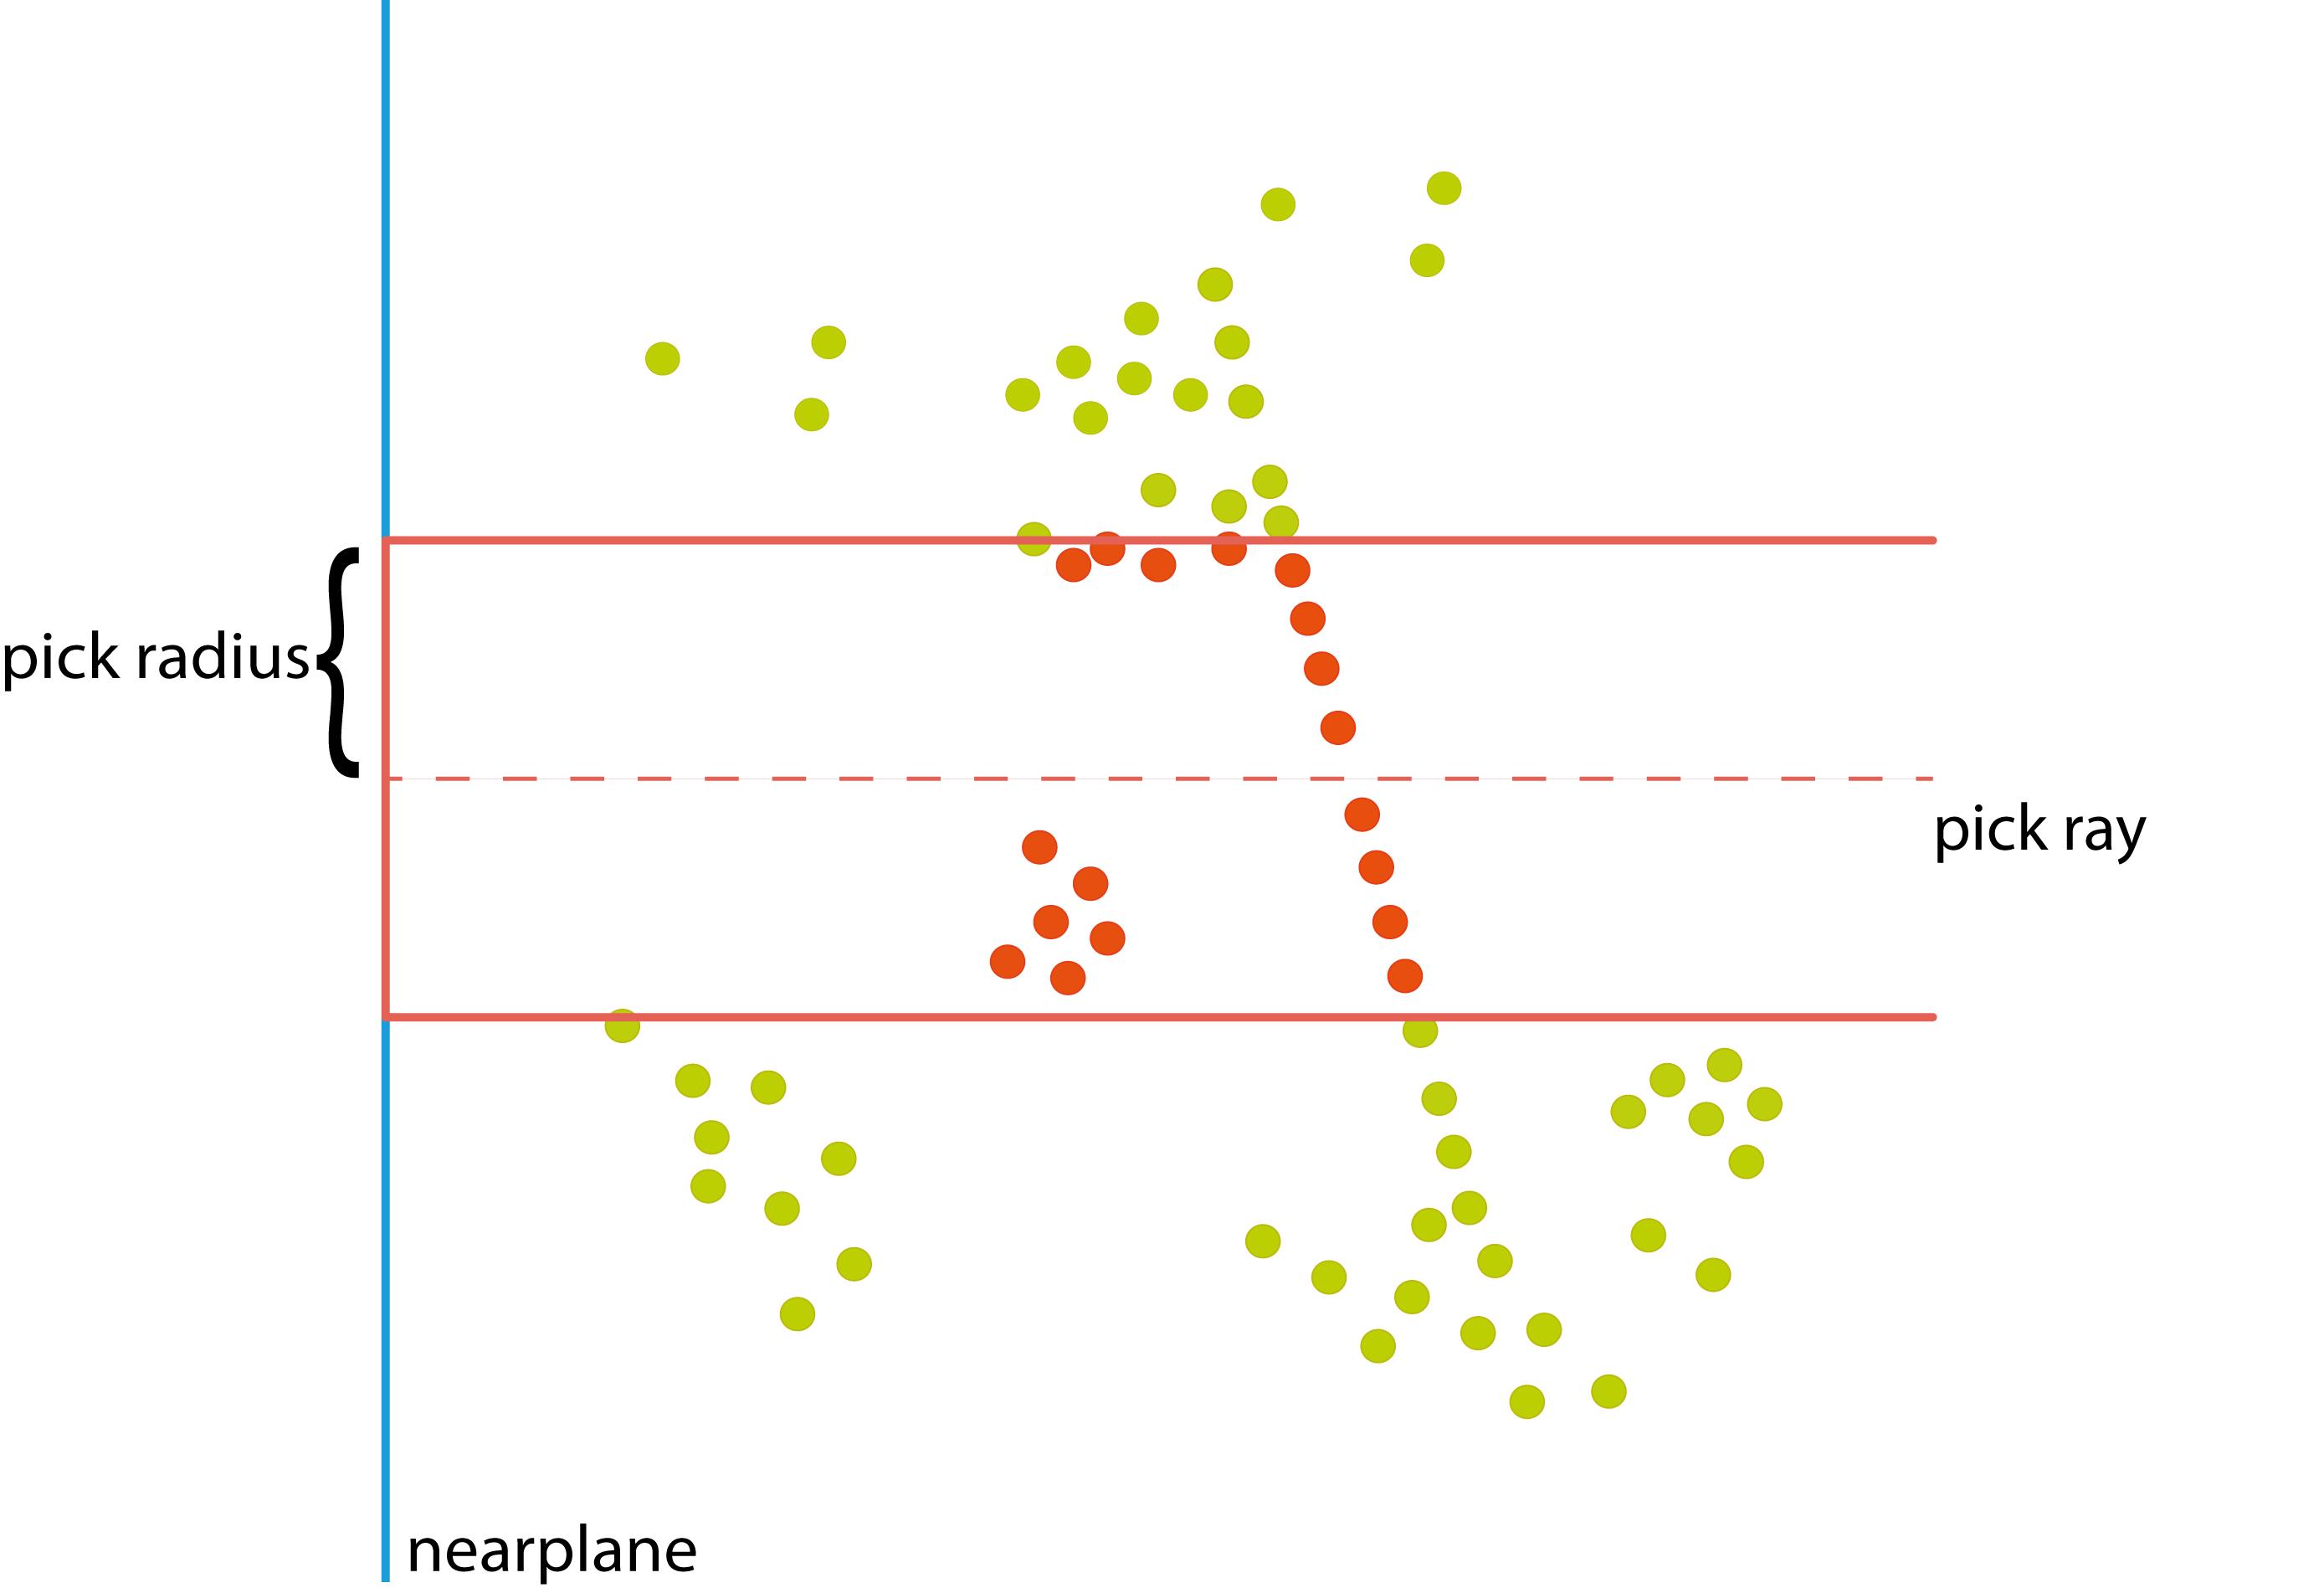
\includegraphics[width=0.6\textwidth]{Interactions/picking_raycast.png}%7
  }\par\medskip
\subcaptionbox{ \label{fig:picking_conecast}}{%
  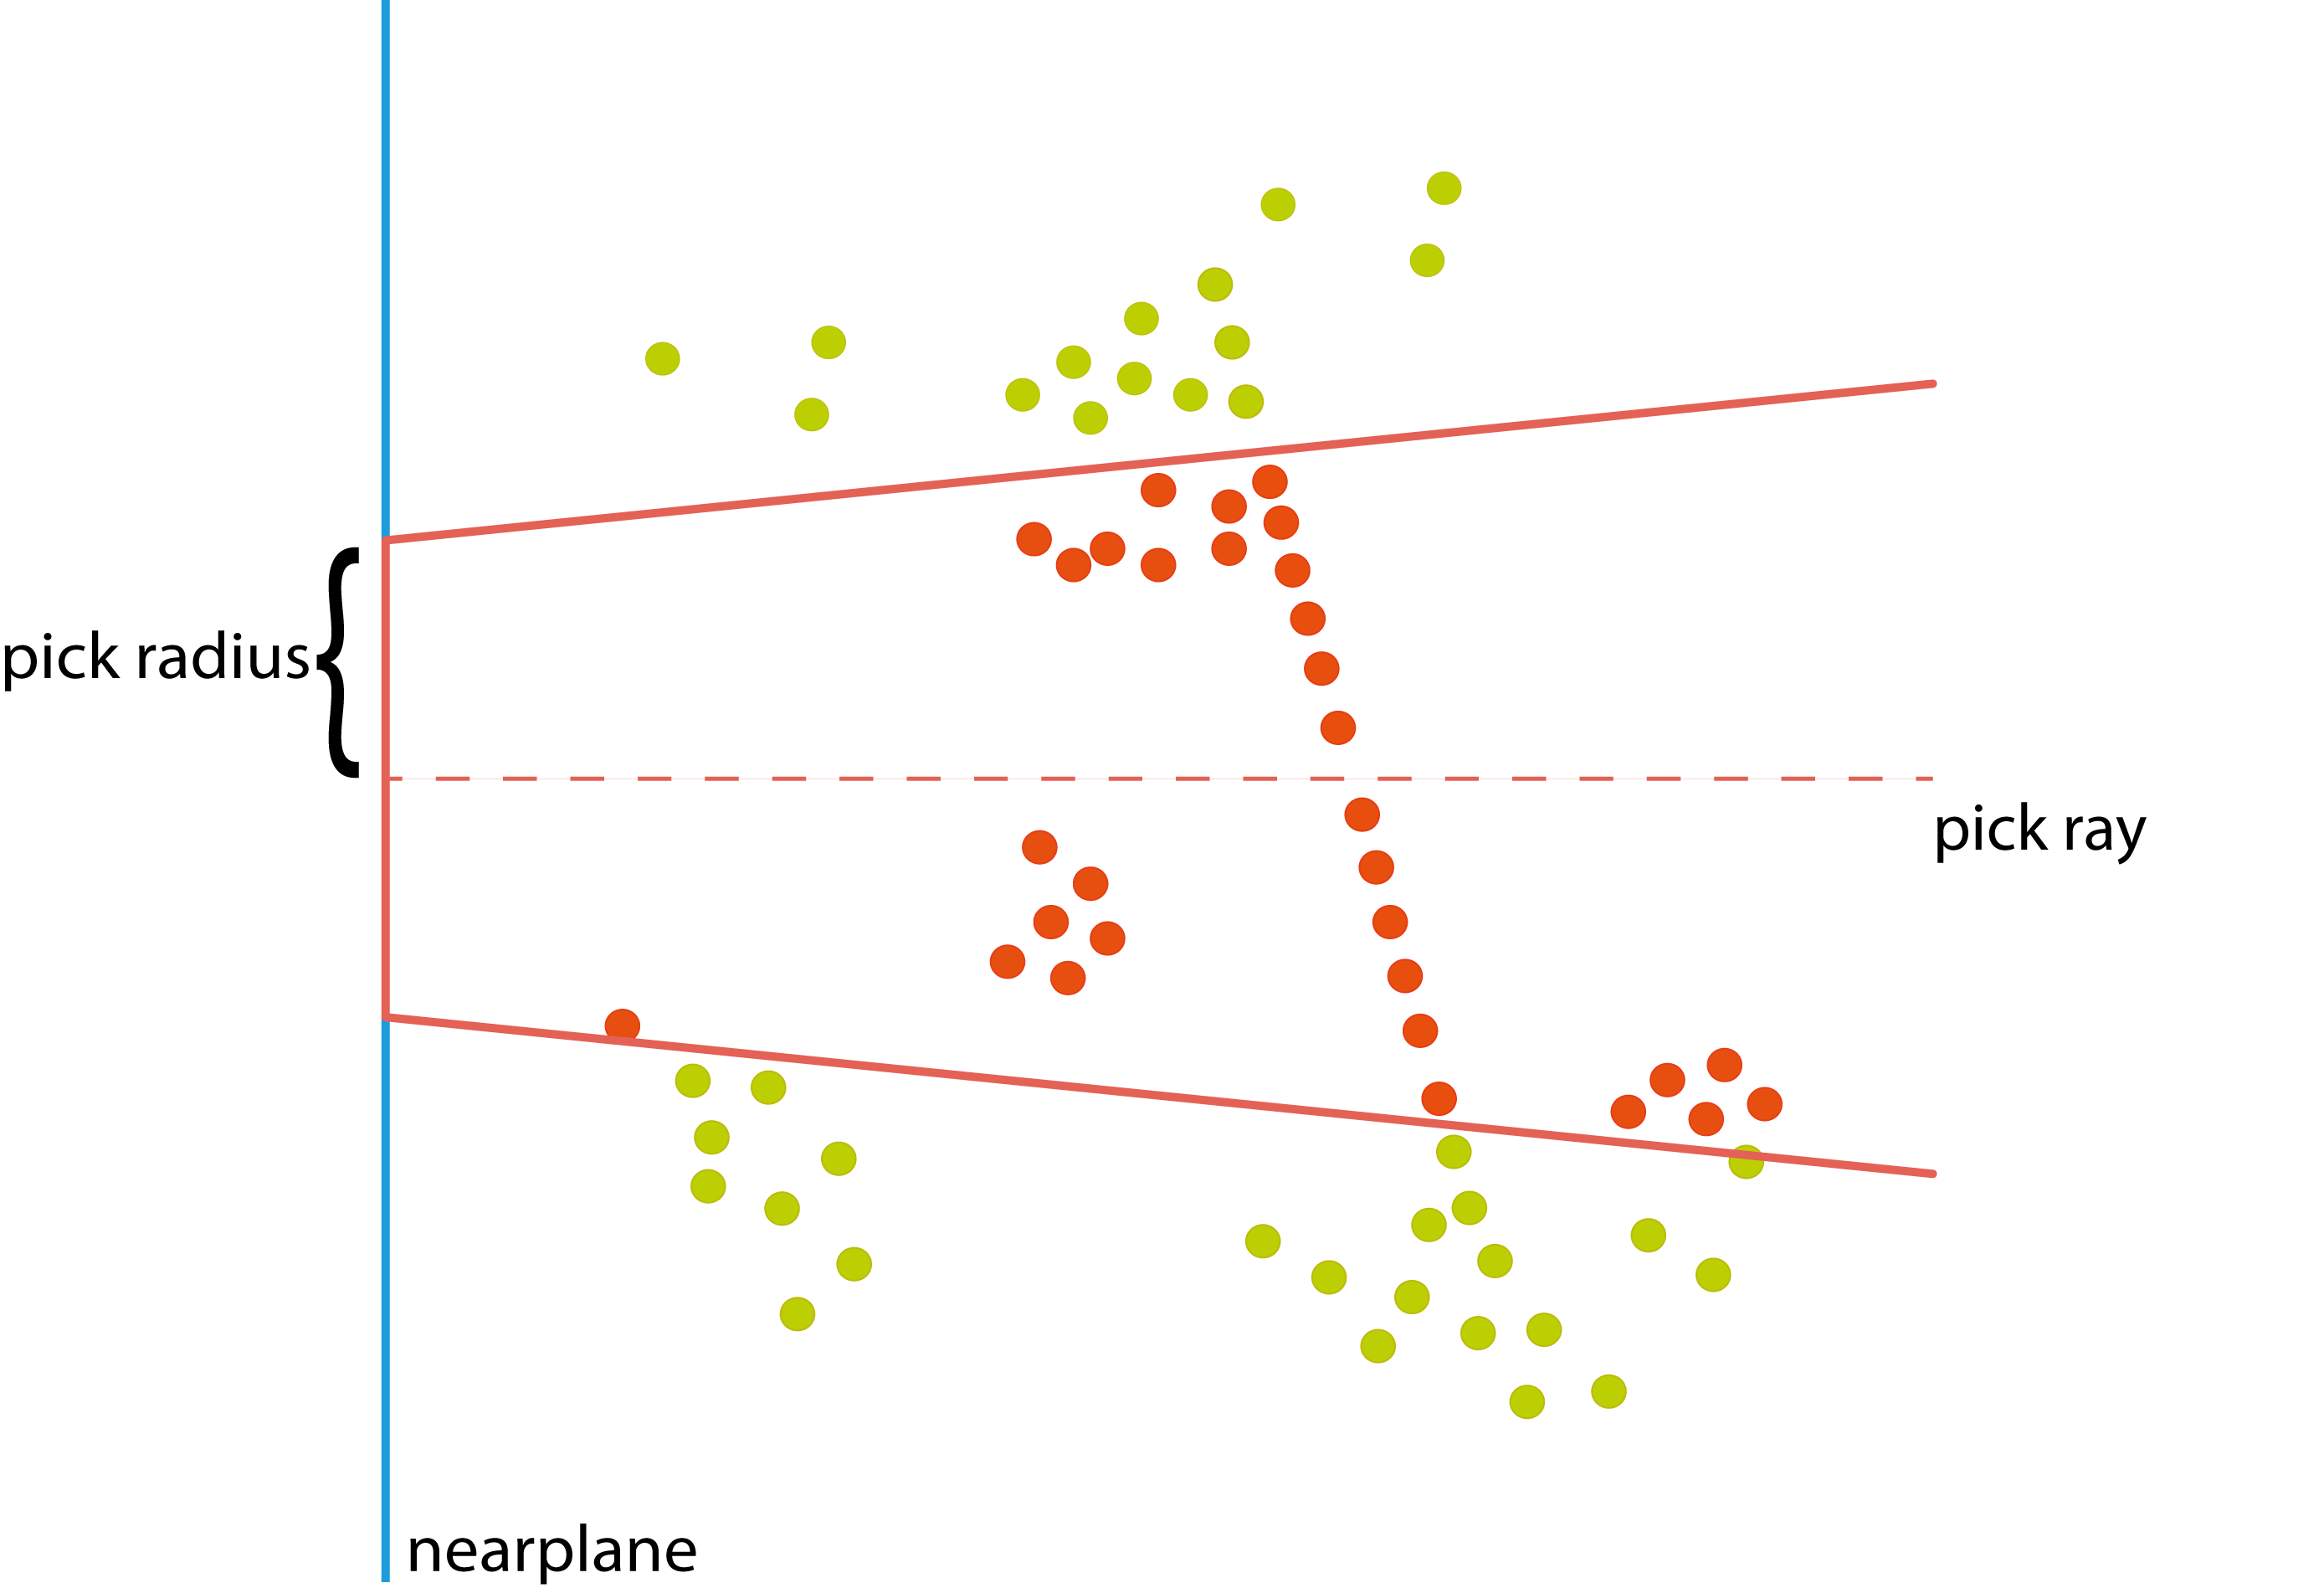
\includegraphics[width=0.6\textwidth]{Interactions/picking_conecast.png}%
  }\par\medskip        
\subcaptionbox{ \label{fig:picking_assisted}}{%
  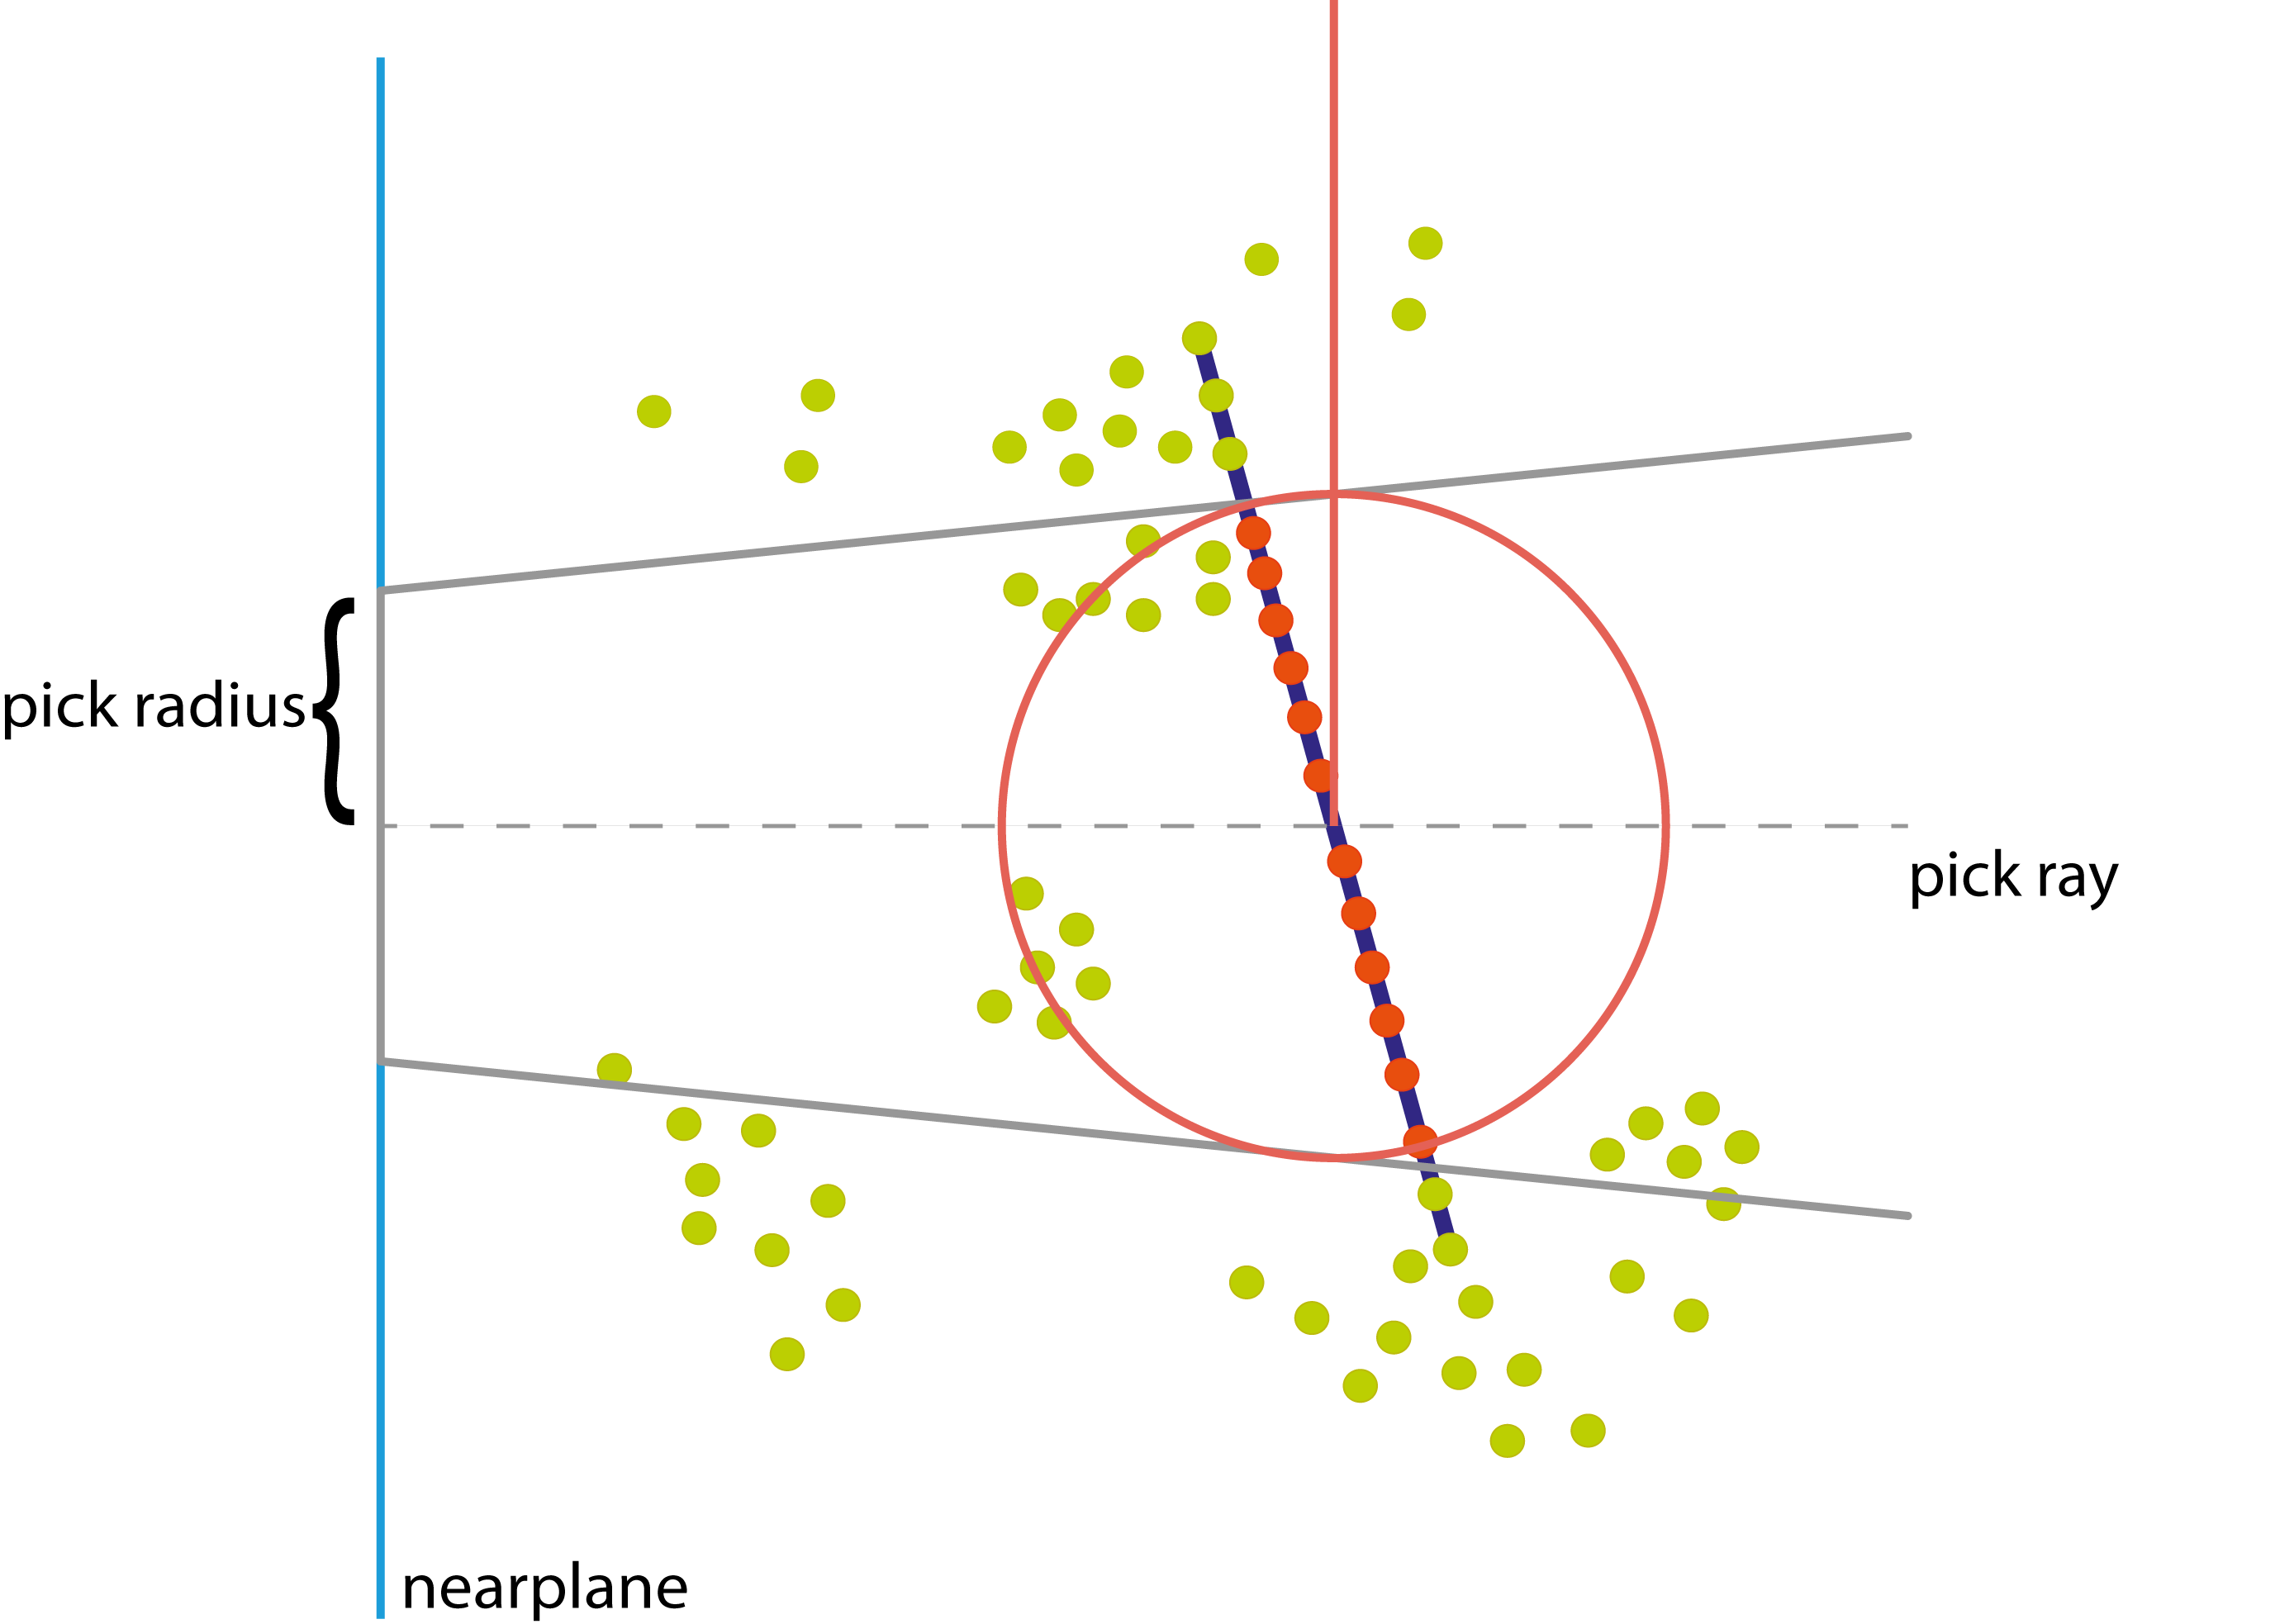
\includegraphics[width=0.6\textwidth]{Interactions/picking_assisted.png}%
  }
\caption{Two-dimensional illustration of various picking methods. Candidate points are colored in green, other points are colored in red. The areas in red describe the different volumes in which candidate points are located. (a) showcases a picking process using a simple raycast. The ray combined with a radius constructs a cylinder in world space which contains all candidate points, (b) uses a cone instead. (c) utilizes a selected shape (dark blue) in order to further filter the candidate points to only follow the curvature of the shape. A spherecast is then performed on the filtered points using the unprojected pick radius as radius to select the final set of candidate points. }
\label{fig:picking}
\end{figure}


\section{Region Selection}

Region Selection aims to not pick a single point at once, but select a set of points, that are spatial neighbors
The design for the \textit{Shape-Assisted Region Selection} is guided by one seemingly simple example task: \textit{Select points that belong to this wall only}. A wall can intersect with other building elements such as roof, balconies or the ground. In regions close to intersections, it is tedious and cumbersome to only select points on the desired structure. Using two-dimensional interaction metaphors, selecting spatially neighboring points along the same curvature, is particularly challenging, since the system does not know the desired depth boundaries for the selection region. In this chapter the benefits of using support shapes for two- and three-dimensional interaction metaphor are discussed. 


\subsection{Volumetric Brush}

The \textit{Volumetric Brush} by Weyrich et. al\cite{weyrich2004post} is designed in such a way that a volume is projected onto the foremost geometry. Points that intersect this volume are considered to be selected. To retrieve the projected position of the volume, usually a sphere, the depth buffer is consulted and the depth value for the current mouse position is retrieved. The world position is the unprojection of the mouse position's $xy$-coordinates and the depth value. 
\\
Since this technique follows the foremost geometry only, sudden depth changes occur if the area of interest is occluded by different geometry. Thus view changes are still required to achieve the example task. In regions close to intersections with other structures, such as below the roof, the user must control the size of the volume in order to not select points on neighboring structures. 


\subsection{Lasso Selection}

The \textit{Lasso Selection} is a common two-dimensional interaction metaphor used for multiple geometry-based applications. While it is an effective technique to selected regions in 2D, drawbacks appear when porting the interaction to 3D. The user draws a polygon onto the screen. All points, whose projection lie inside this polygon, are selected. Much like \textit{Point Picking}, points are projected onto the nearplane and and the intersection between the point and the polygon determines if the point is selected. The combination of a two-dimensional polygon and the projection of points describes an three-dimensional area. The polygon is extruded in the view direction up to a user-defined distance. All points that lie within this volume are selected. Figure \ref{fig:lasso_sketch} showcases the volume created by a lasso polygon drawn onto the screen.


\begin{figure}
	\centering
	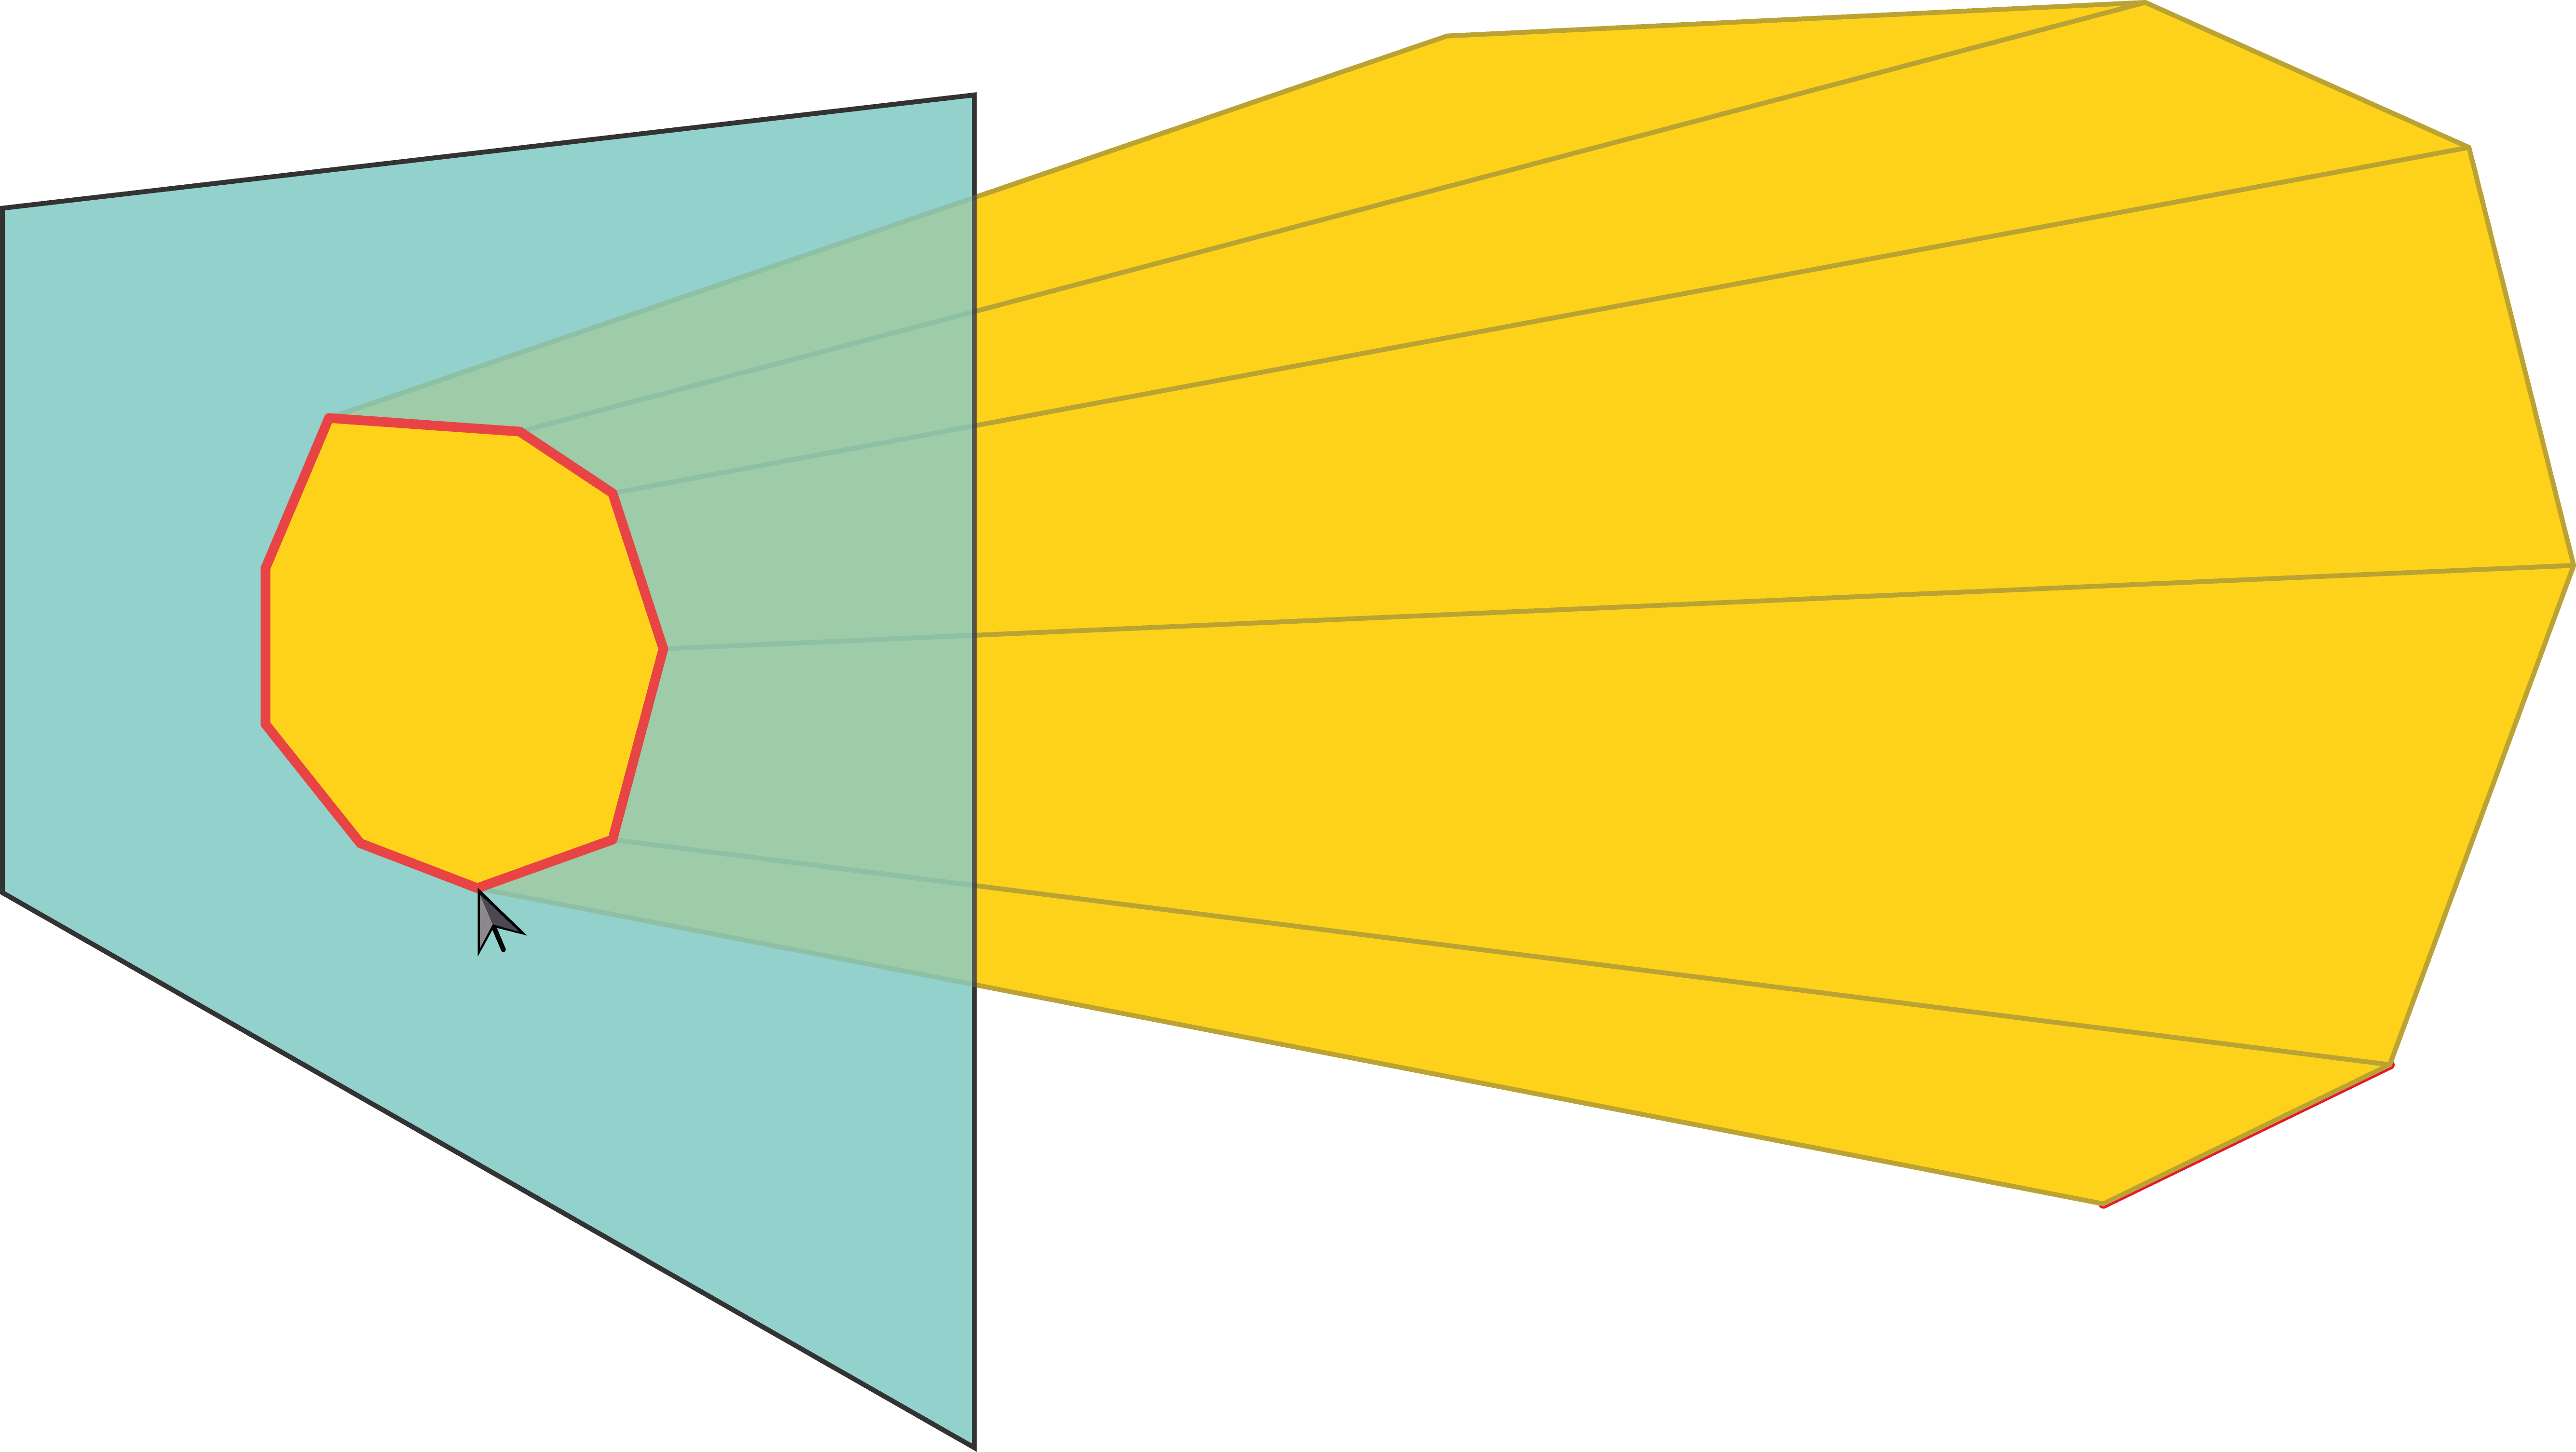
\includegraphics[width=0.8\textwidth]{Interactions/lasso_sketch.png}%7
	\caption{The user draws a polygon(red) on the screen(light blue). The constructed three-dimensional area(yellow) contains all points, whose projection lie inside the lasso polygon. }
	\label{fig:lasso_sketch}
\end{figure}


\begin{figure}
\centering
\subcaptionbox{ \label{fig:lasso1}}{%
  \includegraphics[width=0.5\textwidth]{Interactions/lasso1.png}%7
  }\par\medskip
\subcaptionbox{ \label{fig:lasso2}}{%
  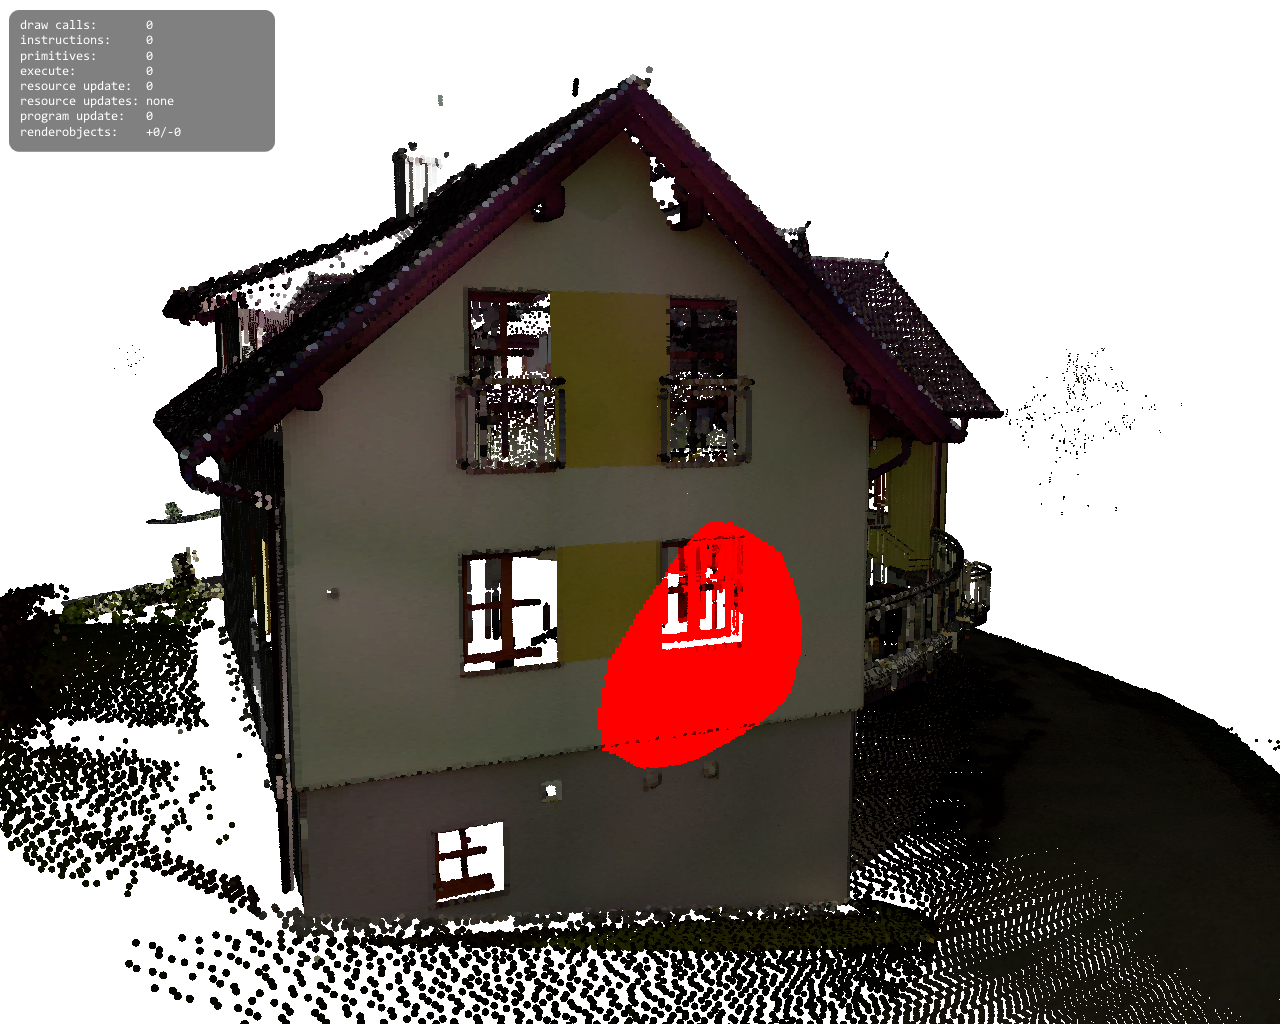
\includegraphics[width=0.5\textwidth]{Interactions/lasso2.png}%
  }\par\medskip        
\subcaptionbox{ \label{fig:lasso3}}{%
  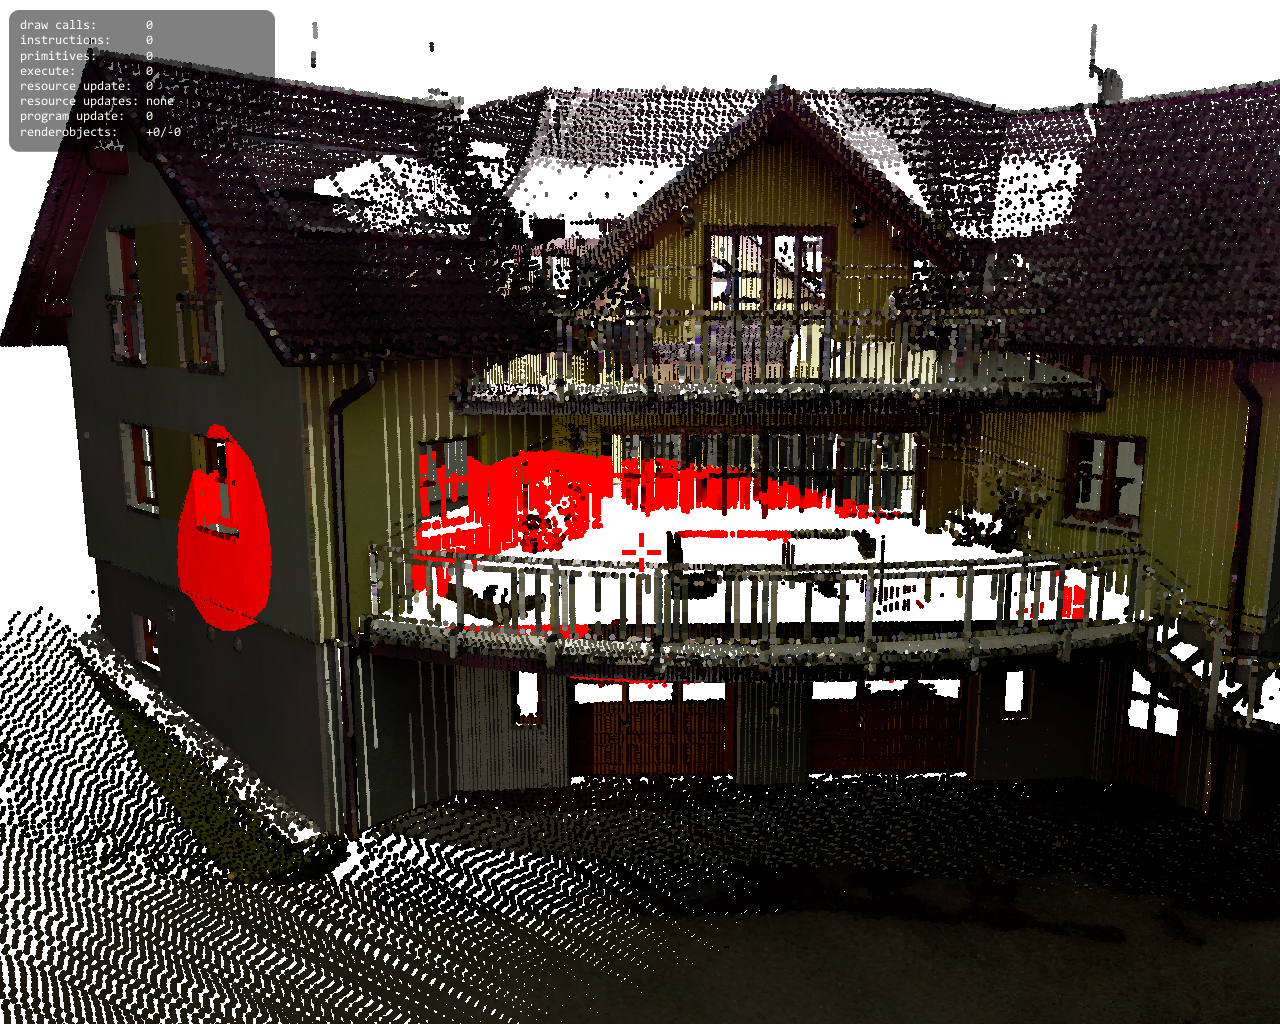
\includegraphics[width=0.5\textwidth]{Interactions/lasso3.png}%
  }
	
\caption{(a) - (c) show a lasso selection performed on a point cloud. In (a) the user draws a polygon onto the screen. In (b) the selected points are visualized in red. Figure (c) showcases the selection from a different angle. All points that are projected to the area of the polygon, are selected. This results in the unintentional selection of points that are obscured by objects in the foreground.}
\label{fig:lasso}
\end{figure}


Figure \ref{fig:lasso} shows a lasso selection performed on a point cloud. The user draws a polygon onto the screen. The selected points are highlighted in red. When changing the view, selected points that where occluded when drawing the lasso, appear. The user must control the selection distance by hand in order to minimize this effect. However, the in order to solve the task of only selecting points on the wall, further lasso selections must be used to remove points from the selection that where selected unintentionally. 





\subsection{Shape-Assisted Region Selection}
\section{Shape-Assisted Local Level-of-Detail Increase}

\chapter{A functional out-of-core octree}
\section{Overview}
Modern point clouds are often to large too fit into memory, let alone video memory. In order to manage datasets whose size exceeds several gigabytes, the data must be stored in an structured way, such that data can be loaded in chunks efficiently. Depending on the camera's view and a level-of-detail ruling, only a subset of points is processed in the memory and displayed. This method is commonly know as out-of-core processing. One common way to introduce structure to point clouds is by storing the data in an octree. 


\section{Out-of-core octree}

An octree is a hierarchical datastructure in which each node represents a spatial region, defined by a 3d bounding box. If the number of elements in a node exceeds a threshold $n$, the node is partitioned into eight children, each representing one octant. If a node is partitioned, it's elements become a random subset of points of size $n$ from it's children, thus creating an efficient level-of-detail representation of the point cloud. 
Other implementations, such as Potree\cite{SCHUETZ-2016-POT}, where some points remain in the parent instead of being stored in a child node, are more efficient in terms of disc space. With our approach, each node can be viewed as self-contained, such that no points from predecessor nodes are needed to fully represent the point cloud for this region and level-of-detail.

Each node contains a set of points whose content is stored on the disc. The data is streamed from a file database into memory on access.


\section{Octree Operations}
	
\subsection{Map}
\subsection{Cull}
\subsection{Insert}


%In an functional program, changes in datastructures or variables are considered mutations and often introduce side-effects and 
%Changes in data structures Mutations of datastructures often introduce side-effects and race conditions. In a parallel environment, multiple threads execute %computations tasks that change the octree. 

\chapter{Shape Detection}
\label{chap:shapeDetection}


\section{Overview}

This thesis utilizes shape detection to automatically detect primitive shapes for small parts of the point cloud at a time. It is designed in such a way that the user receives immediate feedback of local geometry for the region under the mouse cursor. The approach utilizes an automated shape detection algorithm that is capable of detecting different types of primitive shapes. This algorithm is designed to find shapes in point clouds that consist of several million points within minutes. However, when looking at the performance for smaller samples, results can be achieved at interactive time rates. Section \ref{sec:schnabel} describes the shape detection algorithm in detail. 
\\

Before using the detected shapes for rendering or interactions, the shapes must be postprocesssed. Since some of the shapes are of infinite size, they need to be refitted to encapsulate the corresponding support points and create a minimal boundary. Section \ref{sec:Refitting} describes this task. 
\\

Section \ref{sec:shapeMatching} proposes a set of heuristics to determine if detected primitive shapes originate from the same geometric structure. Section \ref{sec:shapeClustering} explains the usage of this heuristics in order to create larger, homogeneous cluster of shapes, used for interactions. 


\section{Efficient RANSAC for Point-Cloud Shape Detection}
\label{sec:schnabel}

The section gives a brief overview over the algorithm used to detect primitive shapes. 
Schnabel et al. \cite{schnabel-2007-efficient} propose an automated way to detect simple primitive shapes in unstructured point clouds. The point cloud is decomposed into a set of shapes and a set of unused points. The algorithm supports detection of planes, spheres, cylinders, cones, and tori. 

\textbf{RAN}dom \textbf{SA}mpling \textbf{C}onsens (RANSAC) was first discussed by Fischler and Bolles \cite{fischler1981random} as a paradigm for model fitting for image analysis and automated cartography. However, this approach can be generalized for points with an origin other than images. The shape detection utilizes RANSAC to repeatedly take a minimal set of points to build a primitive shape $\Psi$ and checks if the points in the region roughly follow the curvature of the shape. 

\subsection{Minimal sets}

A minimal set describes the set of points that are needed to construct a candidate shape. 
For each type of shape, the following rule applies: A shape is only considered as candidate shape if all points from the minimal set are within a distance $\epsilon$ to the shape and the normal does not deviate from the shape's normal by more than an angle $\alpha$. 

\begin{itemize}
    \item \textbf{Plane}: A plane is constructed from three points $p_0, p_1, p_2$ whose normals do deviate from the plane's normal less than the angle $\alpha$. 
    
    \item \textbf{Sphere}: A sphere is fully defined by two points $p_0, p_1$ with corresponding normal vectors $n_0, n_1$. The center $c$ of the sphere is defined by the midpoint shortest line segment between the parametric lines $p_0 + tn_0$ and $p_1 + sn_1$. The radius is constructed by averaging the distance of $p_0$ and $p1$ to $c$.

    \item \textbf{Cylinder}:
    In order to create a cylinder, a minimal set of two points  $p_0, p_1$ with corresponding normal vectors $n_0, n_1$ is used. The direction $d$ of the axis is established by $d = n_0 \times n_1$. The origin $c$ of the cylinder is created by projecting the parametric lines $p_0 + tn_0$ and $p_1 + sn_1$ onto the plane $d \cdot x = 0$ and taking their intersection as origin $c$. The radius is the shortest distance between $p_0$ and the axis $c + ud$
    
    \item \textbf{Cone}:
    For simplicity, the minimal set for a cone consists of three points $p_0, p_1, p_2$, rather than two. For each point-normal pair, a plane is created. The intersection of the three planes defines the apex $c$. To describe the direction of the axis a plane is constructed from the points \{$c +  \frac{p_0 - c}{||p_0 - c||}$, $c +  \frac{p_1 - c}{||p_1 - c||}$, $c +  \frac{p_2 - c}{||p_2 - c||}$\}. The normal of this plane is the direction $d$ of the cone axis. The opening angle is given as $\omega = \frac{\sum_{i}^{max} (p_i - c)\cdot d}{3}$
    
    \item \textbf{Torus}:
    A minimal set of four points with normals is used, one more than theoretically necessary, However, this eases the computation.
    Two possible rotational axis are found by intersecting the four point-normal lines $p_i +  \lambda n_i$\cite{marshall2001robust}. For each axis, a full torus is estimated, and the torus is chosen that causes the smaller error in respect to the four points. The minor radius is found by projecting the points onto a plane that rotates around the axis. A circle is constructed using three points, whose radius is the minor radius of the torus. The major radius is given as the distance from the circle center to the axis. 


\end{itemize} 

\subsection{Score function}
\label{sec:scorefun}
To only use points that roughly follow the curvature of a candidate shape, only points within a distance $\epsilon$ are taken into account. Furthermore, each point must fulfill a score function to be considered a support point of the shape $\Psi$. 
The score function for each point consists of the following: 
\begin{itemize}
    \item The distance between the point and the shape must be smaller than $\epsilon$.
    \item The normal of the point must not deviate from the normal of the shape more than a given angle $\alpha$.
    \item Among all points that fulfill the previous two conditions, only the subset of points, which creates the largest connected component embedded in the shape,  is considered.
\end{itemize}

All points that are within a distance $\epsilon$ are taken into account. However, only those whose normals do not deviate from the normal of the shape more than a given angle $\alpha$ are considered support points. Additionally, the number of support points must exceed a threshold value $n$ for this shape to be valid. 


\subsection{Performance}

\begin{table}
    \centering
    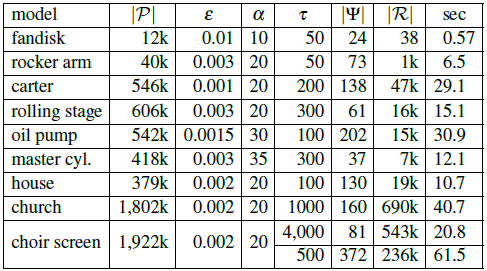
\includegraphics[width=0.7\textwidth]{Shape_Detection/schnabel-performance.png}
    \caption[Original statistics of the shape detection algorithm by Schabel et al.]{The original statistics by Schnabel et al. \cite{schnabel-2007-efficient} on processed models. $\epsilon$ is given as ration of maximum bounding box with. Results have been averaged over 5 runs and rounded.}
    \label{table:schnabel_performance}
\end{table}

Table \ref{table:schnabel_performance} describes the statistical results for different models. $|P|$ is the number of points, $\epsilon$ the distance threshold, $\alpha$ the maximum normals deviation, $\tau$ is the minimum number of support points, $\|Psi|$ the number of shapes found, $|R|$ the number of RANSAC iterations. It can be seen that for small a small number of points and weaker constraints the algorithm returns plausible results within a fraction of a second. We utilize this feature the detect shapes in our application for small regions at a time to give immediate feedback to the user. 


\section{Refitting}
\label{sec:Refitting}

Planes, cylinder, and cones are infinite shapes. Therefore, to use those shapes for rendering and interactions, it is necessary to create finite representations for each shape. Each shape comes with the corresponding set of support points that are used to refit the shape. Spheres and Tori are finite by definition. Therefore they do not require refitting. 


\subsection{Refitting planes}

Planes, however, are represented by a point and a vector. All support points are projected onto the plane, thus reducing the fitting problem to two dimensions. The procedure starts by computing the convex hull of the projected points with the help of Andrew's monotone chain 2d convex hull algorithm\cite{andrew1979another}. 
More complex polygons can be computed. However, for this purpose, a quad is sufficient. The quad is obtained by using the minimum-bounding-rectangle algorithm by Freeman\cite{freeman1975determining}. 


\subsection{Refitting cylinder}

A cylinder is defined by a center $p$, direction vector $v$ and a radius $r$. The height of the cylinder is chosen as the maximum distance between two support points on the axis of the cylinder. This is achieved by projecting all points onto the axis $a = p + vt$ of the cylinder, and select the points $p_{min}$, where $t$ is minimum and $p_{max}$, where $t$ is maximum. The distance $d$ between $p_{min}$ and $p_{max}$ is the height of the enclosing cylinder. The cylinder is refitted such that the new center is set to $p' = p_{min}$ and the $d$ is encoded in the length of the new direction vector:$v' = \frac{v}{|v|}d$. The radius stays the same. 


\subsection{Refitting cones}

A cone is defined by its apex $c$, axis direction $v$, and opening angle $\theta$. Similar to the cylinder, all support points are projected onto the axis and the points $p_{min}, p_{max}$, with minimum and maximum $t$, are selected. Since the apex of a cone is fixed, the range cannot be encoded using $c$ and $v$. The range is stored separately. Range checks are performed when rendering or interacting with cones. 


\section{Shape Detection Parameter Selection}
\label{sec:shapeDetectionParameterSelection}

This section briefly discusses the issue of selecting optimal parameters for the shape detection. The $\epsilon$ parameter creates an $\epsilon$-band that follows the curvature of the shape. All points within this $\epsilon$ band are considered to be candidates. The authors propose to use the point cloud's bounding boxes largest dimension times $0.1$ as $\epsilon$. However, using such a static parameter yields problems with extremely sparse regions and regions that are populated very densely. In this thesis, shape detection is performed dynamically on local regions of the point cloud at a time. The local density of an octree node is chosen as $\epsilon$. The density is calculated per octree node by averaging the distance of each point to its nearest neighbor. Thus, nodes that are populated more densely create finer geometry. 

The $\alpha$ parameter is used to determine the deviation between two directions. As the normals are the same at different level-of-detail, this parameter is static. We use an $\alpha$ value of $0.95$. 

The minimum number of support points per shape is set to $250$.
\chapter{Interactions}

Creating new interactions is a key topic for this thesis. This chapter describes the pros and cons of current state-of-the-art two-dimensional interactions and proposes improvements using the detected primitive shapes as interaction support shapes. 

Many proven interaction techniques have emerged over time, such as \textit{Point Picking} or \textit{Region Selection}. 

%% TODO: define pick ray
%% TODO: define candidate global
%% TODO: define point belongs to a shape

\section{Shape Picking}


\section{Point Picking}
\label{sec:picking}
\textit{Point Picking} describes an interaction, where the user is interested in selecting a single point from the scene at a time. A \textit{pick ray} describes a ray originating from the mouse position whose direction is the view direction. The pick radius $r$ denotes the maximum distance of a point to the pick ray in order for the point to be considered a candidate point. Depending on the use case the pick radius $r$ can be depended on the depth value. There are multiple ways of implementing this interaction with varying results. 
\\
\\
The first explored technique is to use a fixed pick radius in world space. The picked point is the point closest to the pick ray in world space. Since the user only interacts with points that are projected onto the nearplane, the projection of the pick radius is smaller for points that lie in the background. Therefore, the distance in pixel between the mouse position and a picked point in the background is smaller than the distance to a picked point in the foreground. While this encourages the picking of points in the foreground, the non-uniform pixel distance introduces inconsistencies. 
\\
\\
A more consistent way of picking a point is to only use the screen space information for each point. The mouse position $p$ in screen space combined with the pick radius $r$ create the pick circle $c$. This circle corresponds to a projection of a cone. All points that intersect this cone are treated as candidate points. In order to calculate this intersection, all points are projected to the screen space. The cone intersects a point if $c$ contains the point in screen space. Then the point with the projection closest to the mouse position is picked. This technique works consistently for different depth values. However, since all points are treated equally, the technique does not distinguish between foreground and background points, thus introducing possible depth ambiguities. 
\\
The projection of points can be executed on the GPU by rendering the projected points, paired with an identifier, to a texture. From this texture, a window around the mouse cursor is downloaded and the closest point is determined. Reading pixels from a texture forces the CPU and GPU to sync and stalls the graphics pipeline. 
\\
\\
The user interacts with points that are presented on the screen only. Moreover, only points are of interest, whose projection on the nearplane lie in close proximity to the mouse position. Since this interaction cannot be computed for all points in real-time, unneeded octree nodes must be filtered beforehand. This prefiltering can easily be achieved by performing a raycast through the octree and collecting all nodes whose bounding boxes intersect the pick ray. However, consider the case, that the pick ray does not intersect a node's bounding box, but the distance of the box to the ray is smaller than the pick radius. Some points might exist that should be considered candidates, but due to the nature of a raycast, are discarded. This introduces the possibility that points that can be the picking result, are not considered, introducing inconsistency to the pick interaction. One solution to overcome this problem is to use a conecast instead. 
\\
A circle on the nearplane is the projection of a cone in world space. The corners of the box are projected onto the nearplane and the convex hull polygon is calculated. The intersection then is determined by the intersection of the polygon with the pick circle $c$. 


\subsection{Shape-Assisted Point Picking}
Picking comes with the disadvantage that some constellations of points can influence the picking interaction in a negative way. Points that occlude structures of interest force the user to change the view in order to pick the desired point. In some cases, a point in the background is favored over a desired point on a structure. 
 \textit{Shape-Assisted Point Picking} utilizes primitive shapes to perform the picking routine only on points that are part of a structure. The user selects a cluster of shapes, thus reducing the amount of possible candidate points to only those that belong to this shape. 
\\
Instead of performing a cone- or raycast on the octree, only those nodes are taken into account, whose bounding boxes intersect the shape cluster. Each point that does not fulfill the score function from Section \ref{sec:scorefun} for the particular canidate shape is discarded as well, leaving only a handful of points on which a conecast is performed. The pick radius in world space is calculated by unprojecting the pick circle to the intersection point of the pick ray with the shape cluster. Only points are considered that lie in the pick sphere, constructed by the intersection point and the pick radius. The point closest to the intersection point is then picked. Due to the curvature of shapes, such as cylinders and spheres, points on the back of a shape are projected in close proximity to the mouse position as well. By using the projected distances, points that lie on the back side of the shape might get favored over points that are on the front side of the shape (facing the user). 
\\

This technique comes not only with interaction benefits, computation time is drastically reduced as well. Usually a shape cluster consists of less nodes than a raycast since the cluster's extension is limited to a region in the point cloud. Points within a node are also reduced such that intersections and distance measures are computed only for candidate points. 

\\
Figure \ref{fig:picking} shows the different picking methods, described in Section \ref{sec:picking}. Figure \ref{fig:picking_raycast} showcases a simple raycast with a radius. The combination of a ray and a radius yields a cylinder, which contains all candidate points on world space. The pick distance in world space is consistent. Figure \ref{fig:picking_conecast} uses a conecast instead. The opening angle is defined by the pick radius in screen space. The pick distance in world space increases the higher the depth value. All points inside the volume are treated equally, introducing consistency in screen space. \Figure\ref {fig:picking_assisted} showcases the use of a support shape to further filter candidate points. All points are filtered that belong to the support shape prior to be used as input for a spherecast. 

\begin{figure}
\centering
\subcaptionbox{ \label{fig:picking_raycast}}{%
  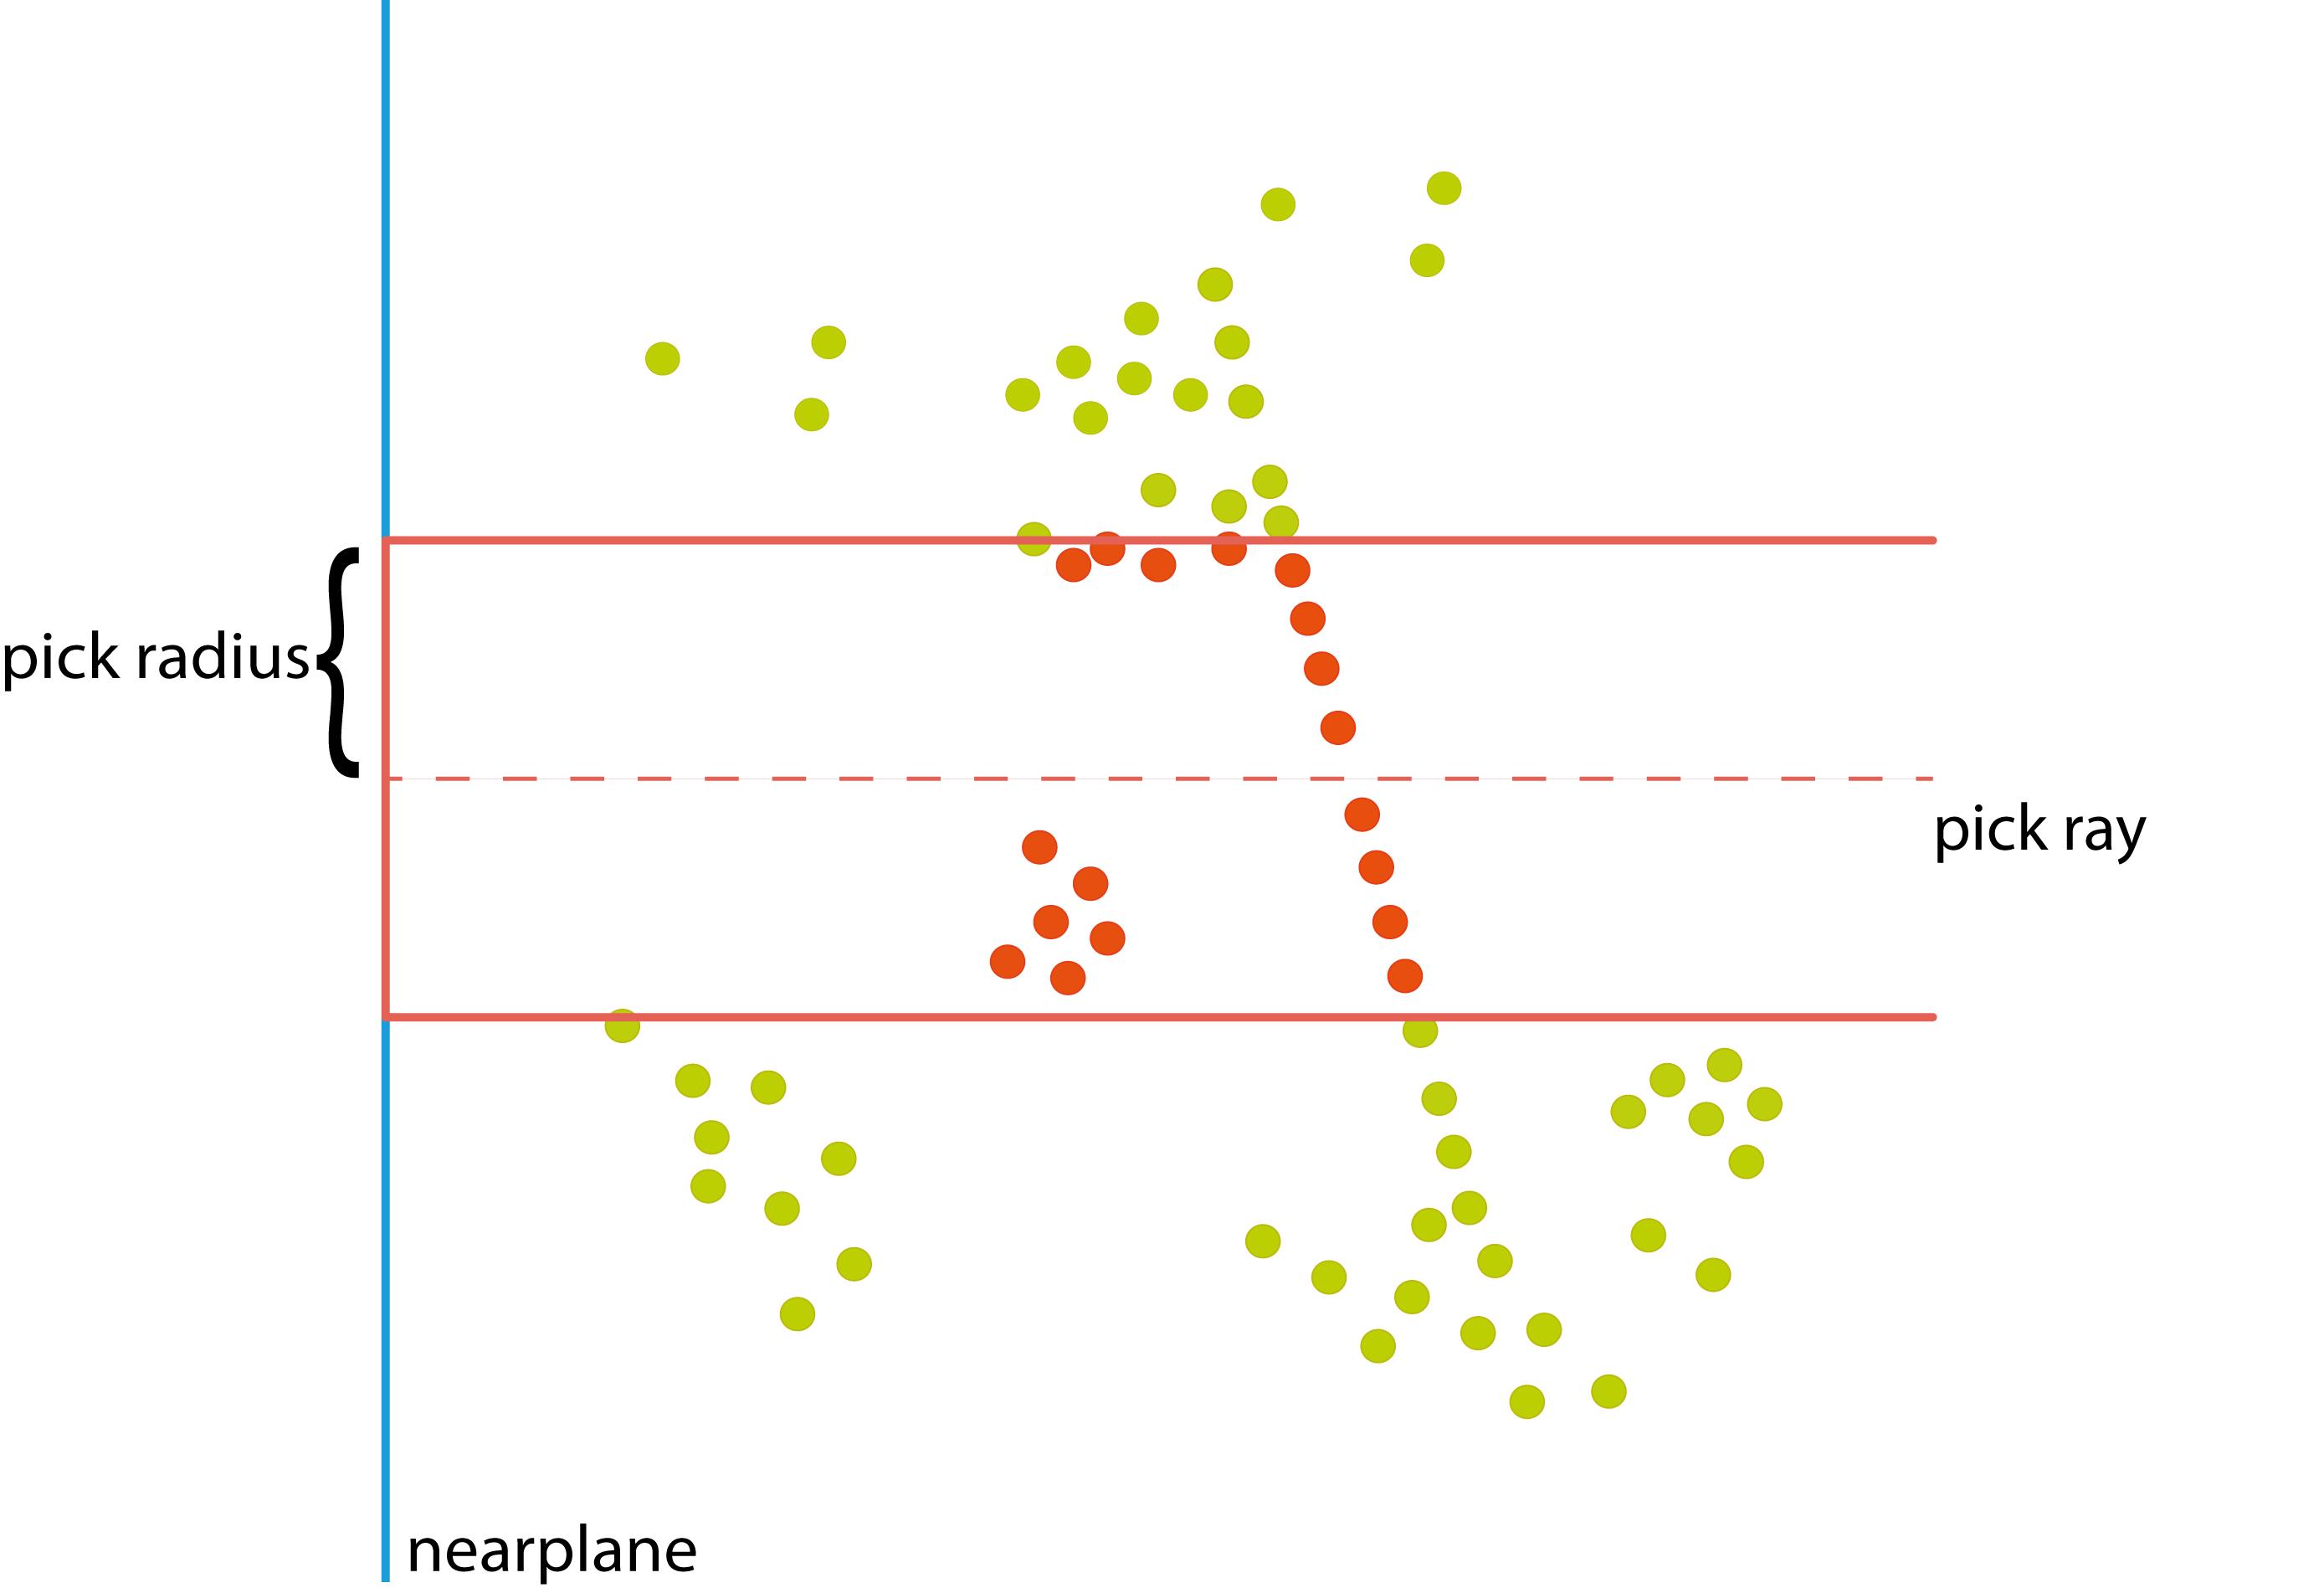
\includegraphics[width=0.6\textwidth]{Interactions/picking_raycast.png}%7
  }\par\medskip
\subcaptionbox{ \label{fig:picking_conecast}}{%
  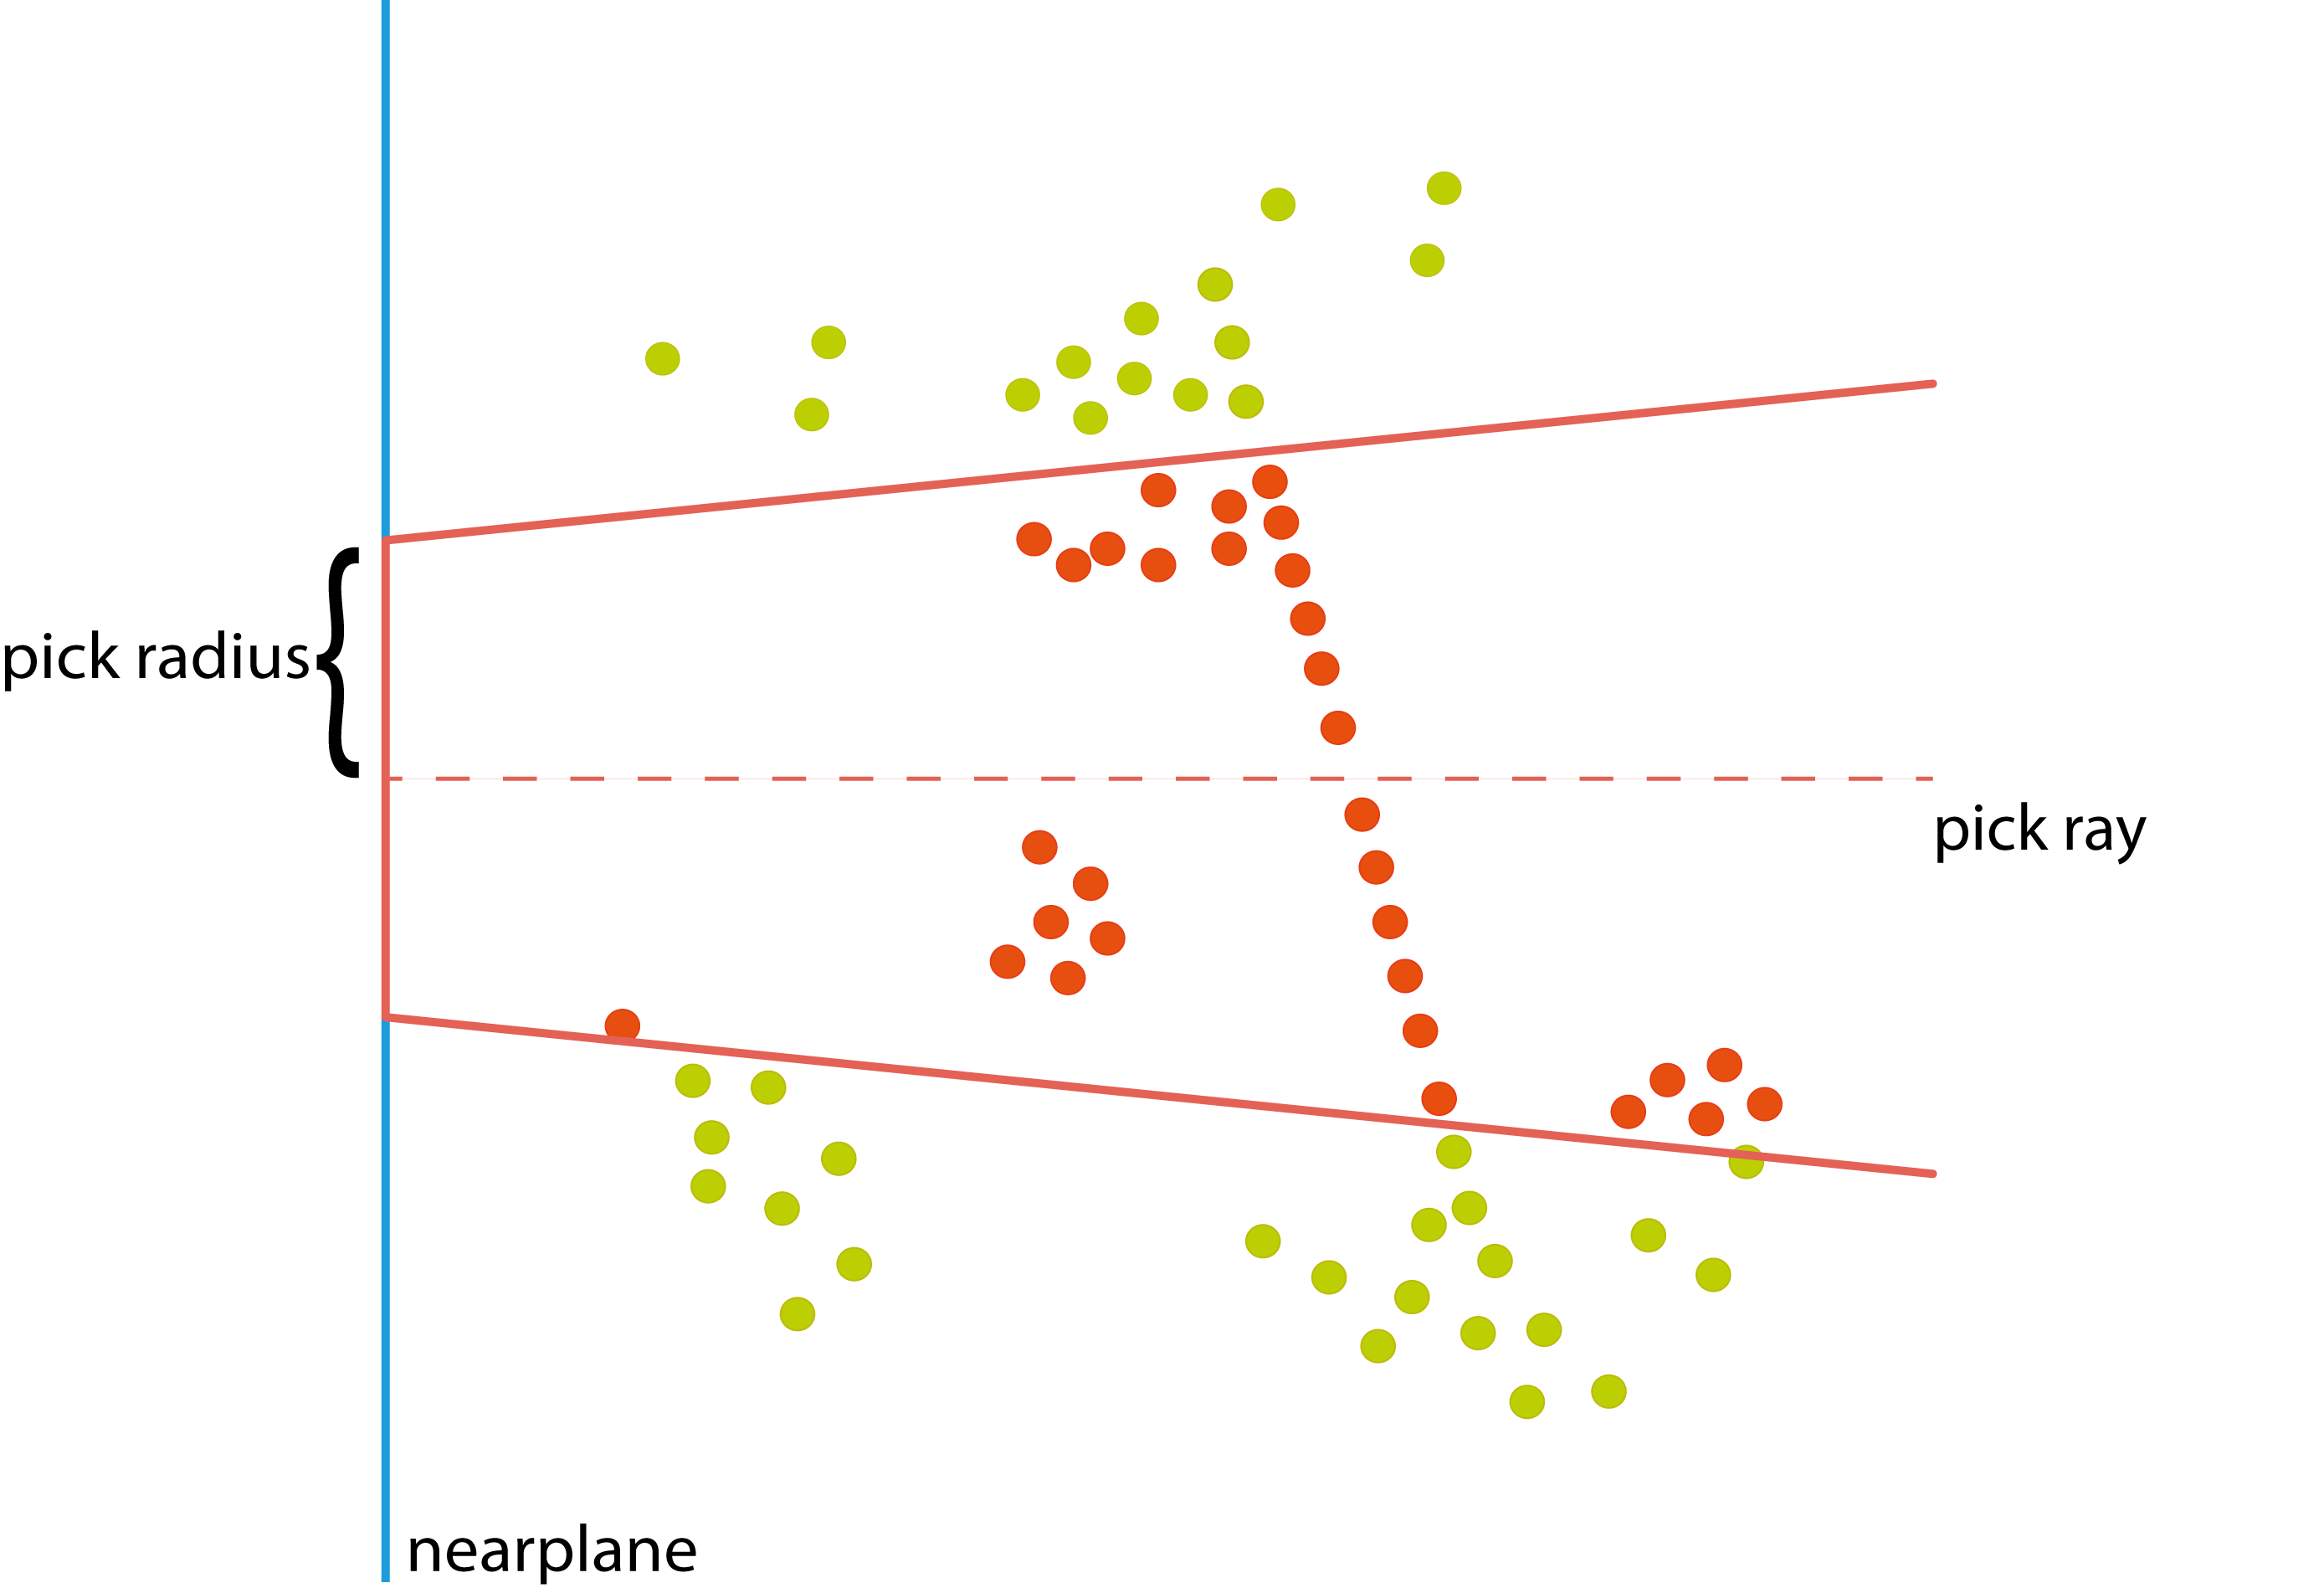
\includegraphics[width=0.6\textwidth]{Interactions/picking_conecast.png}%
  }\par\medskip        
\subcaptionbox{ \label{fig:picking_assisted}}{%
  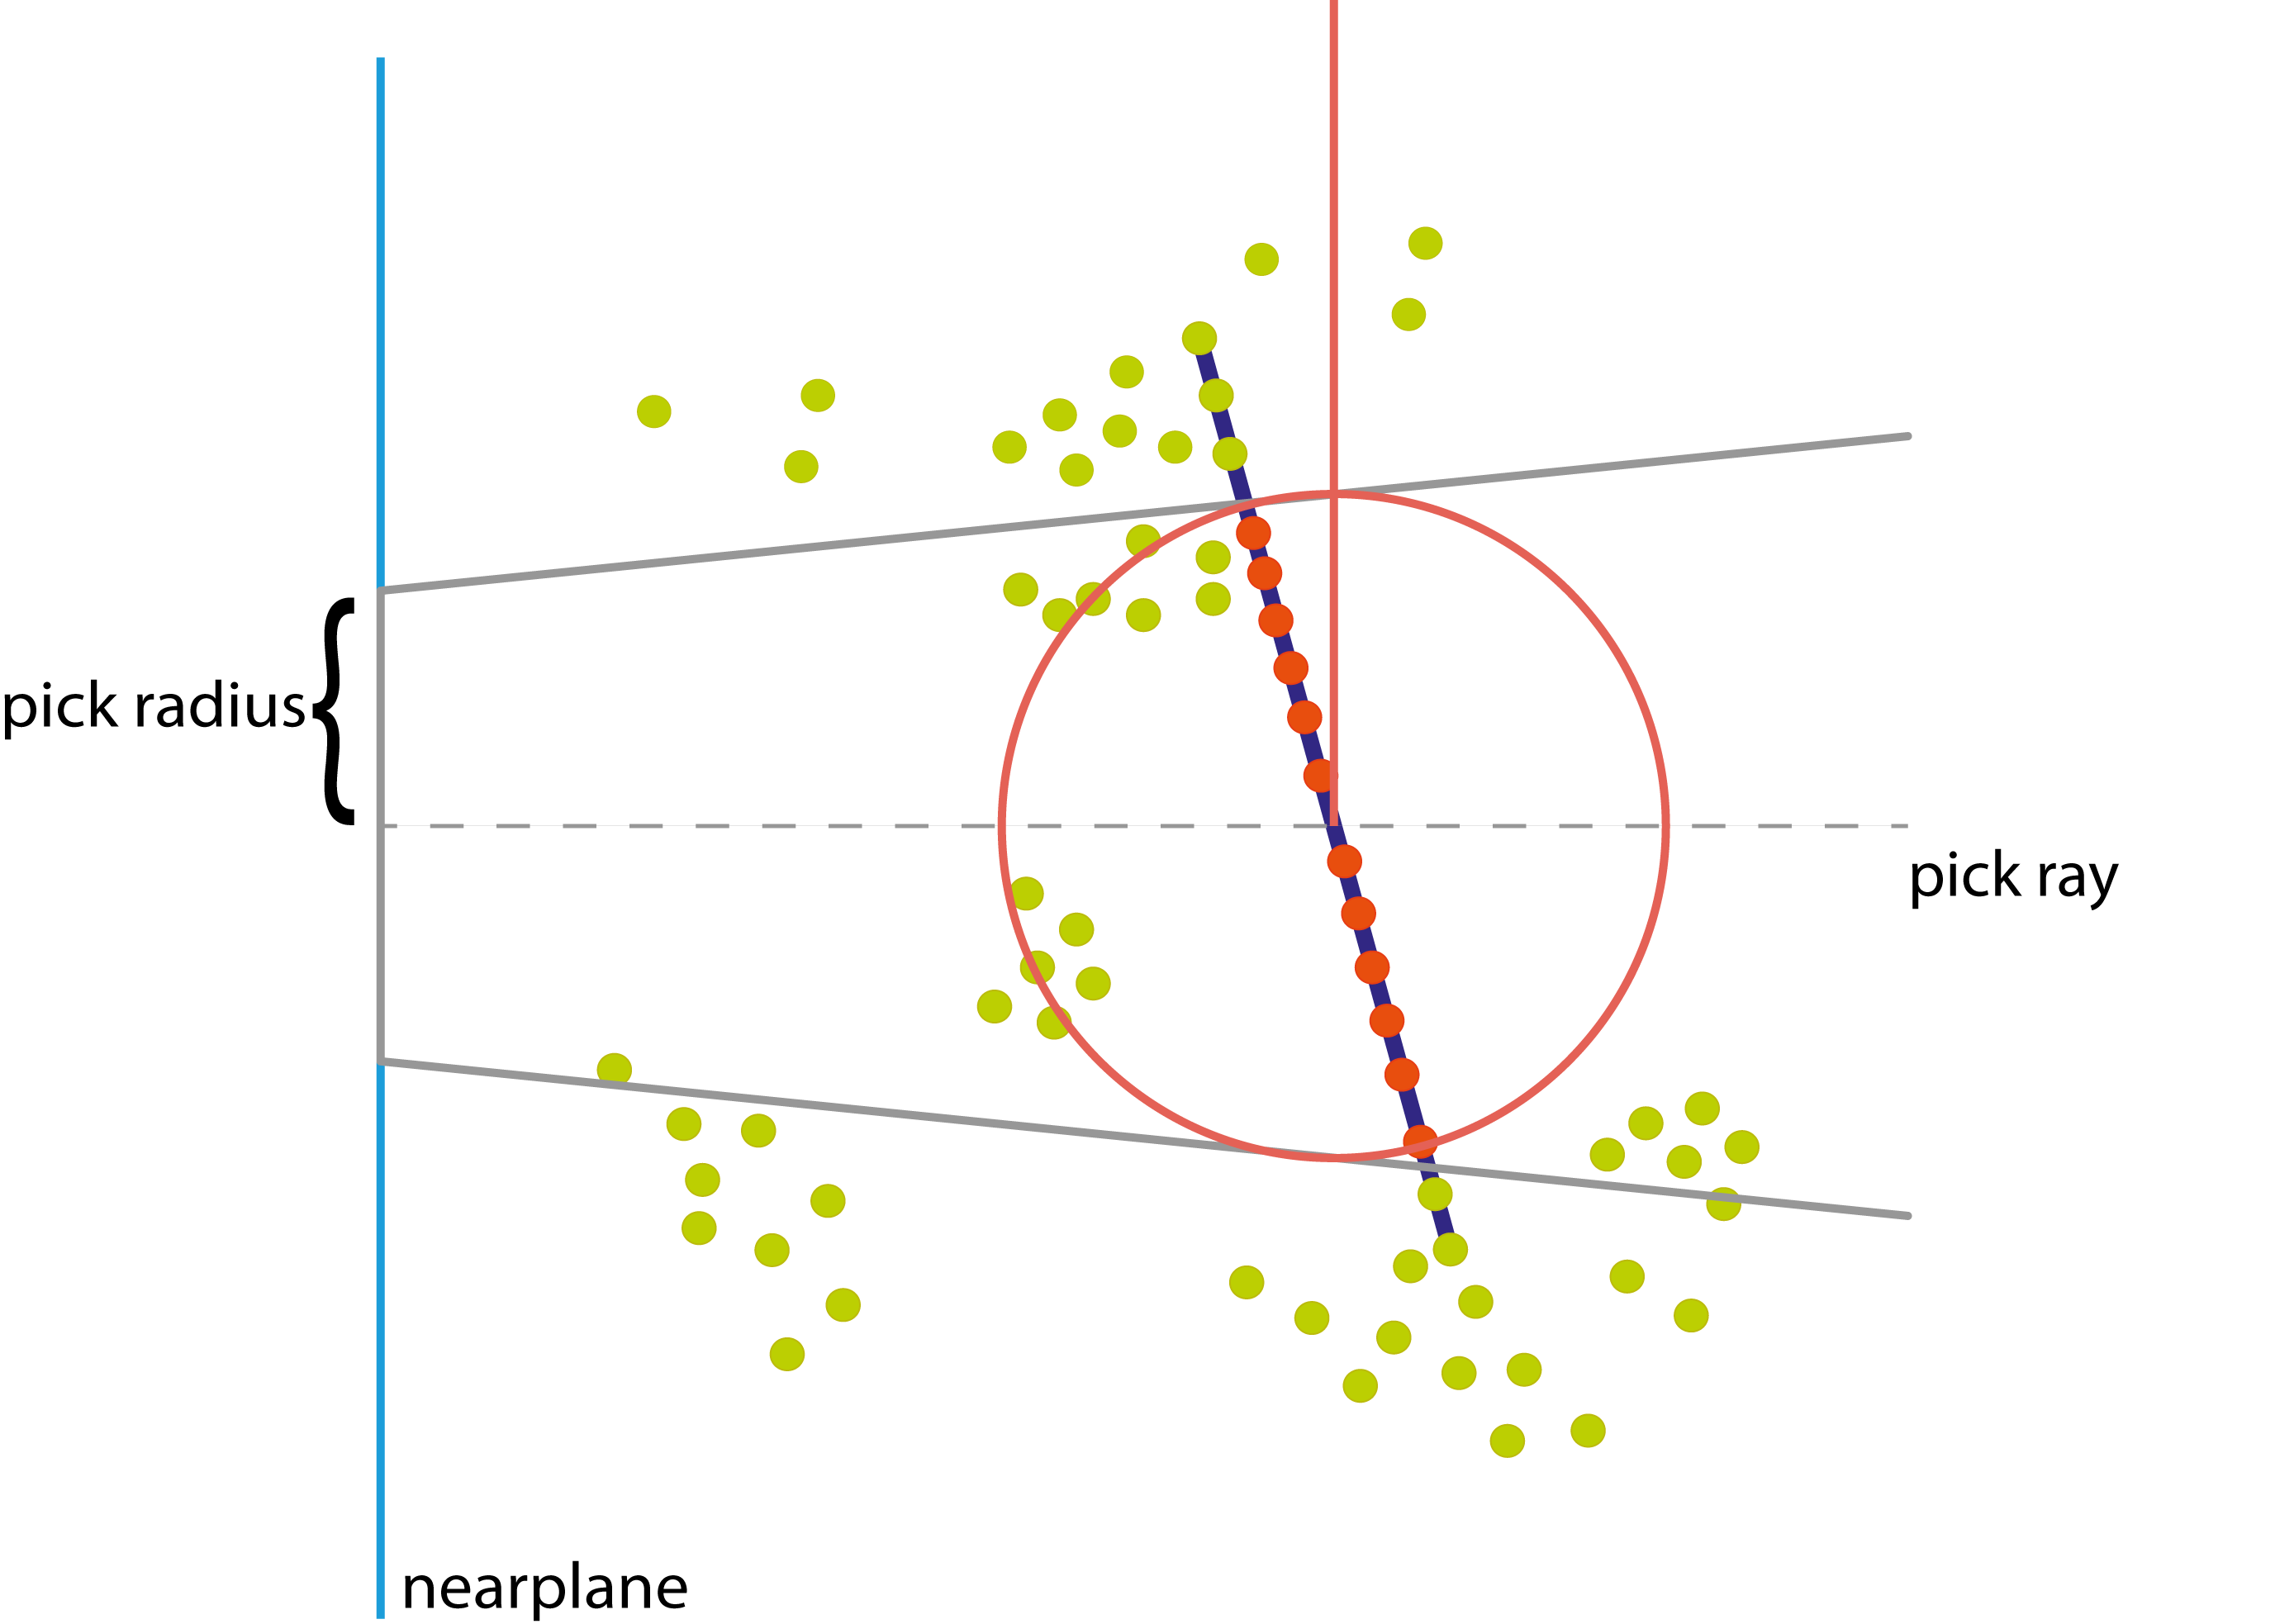
\includegraphics[width=0.6\textwidth]{Interactions/picking_assisted.png}%
  }
\caption{Two-dimensional illustration of various picking methods. Candidate points are colored in green, other points are colored in red. The areas in red describe the different volumes in which candidate points are located. (a) showcases a picking process using a simple raycast. The ray combined with a radius constructs a cylinder in world space which contains all candidate points, (b) uses a cone instead. (c) utilizes a selected shape (dark blue) in order to further filter the candidate points to only follow the curvature of the shape. A spherecast is then performed on the filtered points using the unprojected pick radius as radius to select the final set of candidate points. }
\label{fig:picking}
\end{figure}


\section{Region Selection}

Region Selection aims to not pick a single point at once, but select a set of points, that are spatial neighbors
The design for the \textit{Shape-Assisted Region Selection} is guided by one seemingly simple example task: \textit{Select points that belong to this wall only}. A wall can intersect with other building elements such as roof, balconies or the ground. In regions close to intersections, it is tedious and cumbersome to only select points on the desired structure. Using two-dimensional interaction metaphors, selecting spatially neighboring points along the same curvature, is particularly challenging, since the system does not know the desired depth boundaries for the selection region. In this chapter the benefits of using support shapes for two- and three-dimensional interaction metaphor are discussed. 


\subsection{Volumetric Brush}

The \textit{Volumetric Brush} by Weyrich et. al\cite{weyrich2004post} is designed in such a way that a volume is projected onto the foremost geometry. Points that intersect this volume are considered to be selected. To retrieve the projected position of the volume, usually a sphere, the depth buffer is consulted and the depth value for the current mouse position is retrieved. The world position is the unprojection of the mouse position's $xy$-coordinates and the depth value. 
\\
Since this technique follows the foremost geometry only, sudden depth changes occur if the area of interest is occluded by different geometry. Thus view changes are still required to achieve the example task. In regions close to intersections with other structures, such as below the roof, the user must control the size of the volume in order to not select points on neighboring structures. 


\subsection{Lasso Selection}

The \textit{Lasso Selection} is a common two-dimensional interaction metaphor used for multiple geometry-based applications. While it is an effective technique to selected regions in 2D, drawbacks appear when porting the interaction to 3D. The user draws a polygon onto the screen. All points, whose projection lie inside this polygon, are selected. Much like \textit{Point Picking}, points are projected onto the nearplane and and the intersection between the point and the polygon determines if the point is selected. The combination of a two-dimensional polygon and the projection of points describes an three-dimensional area. The polygon is extruded in the view direction up to a user-defined distance. All points that lie within this volume are selected. Figure \ref{fig:lasso_sketch} showcases the volume created by a lasso polygon drawn onto the screen.


\begin{figure}
	\centering
	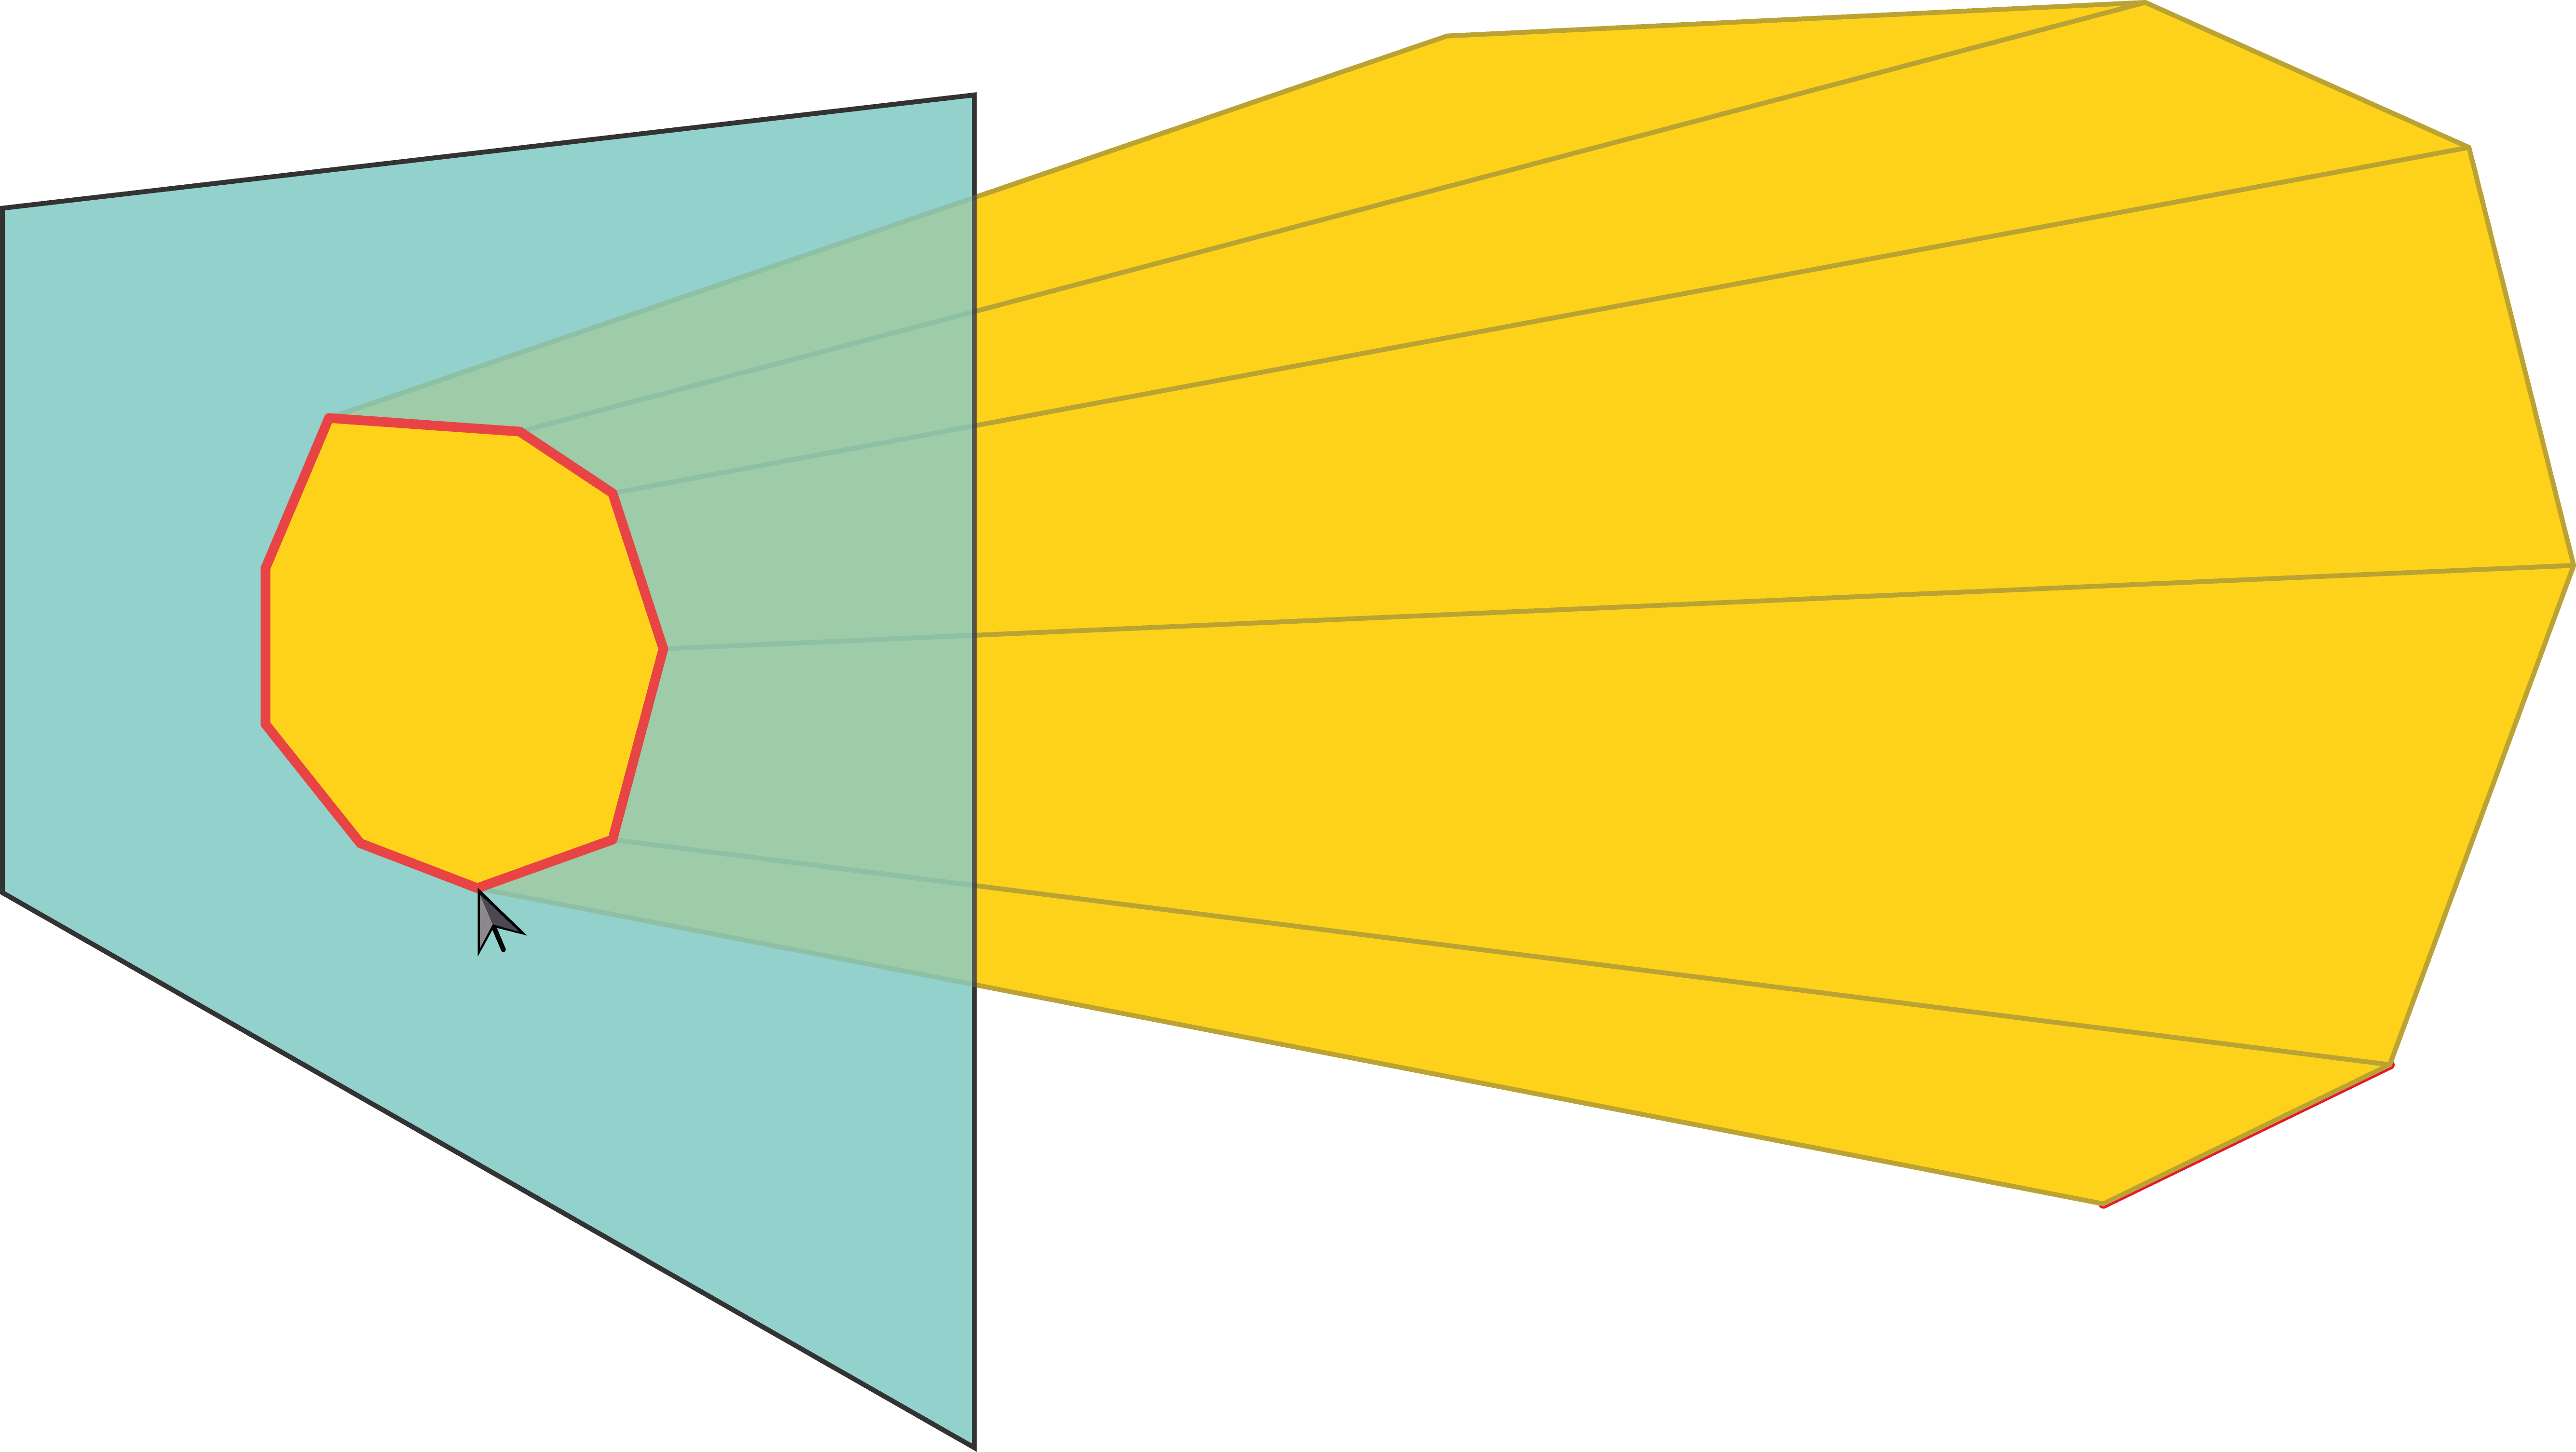
\includegraphics[width=0.8\textwidth]{Interactions/lasso_sketch.png}%7
	\caption{The user draws a polygon(red) on the screen(light blue). The constructed three-dimensional area(yellow) contains all points, whose projection lie inside the lasso polygon. }
	\label{fig:lasso_sketch}
\end{figure}


\begin{figure}
\centering
\subcaptionbox{ \label{fig:lasso1}}{%
  \includegraphics[width=0.5\textwidth]{Interactions/lasso1.png}%7
  }\par\medskip
\subcaptionbox{ \label{fig:lasso2}}{%
  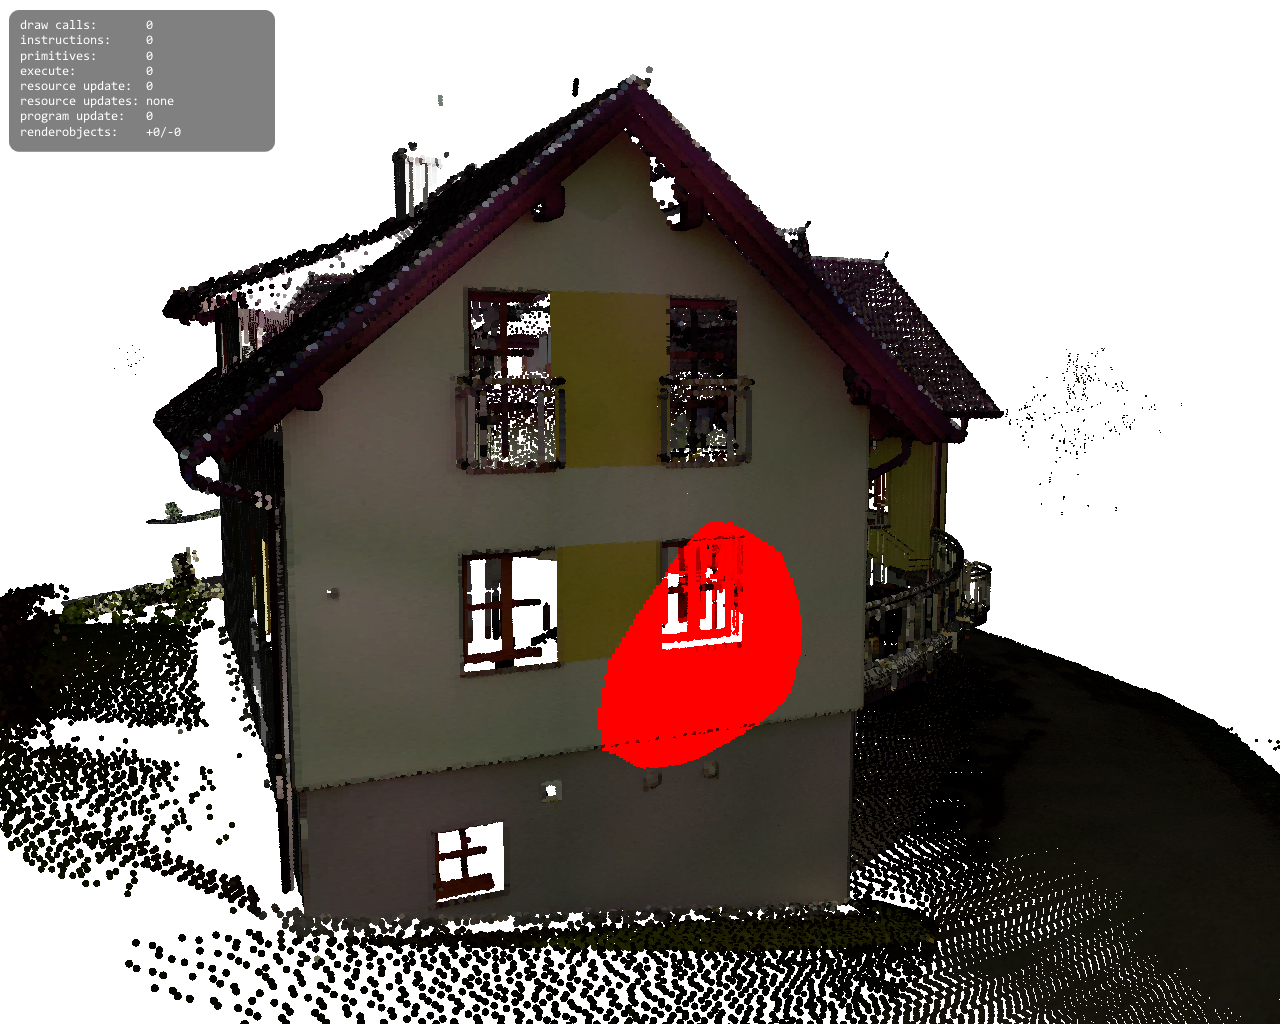
\includegraphics[width=0.5\textwidth]{Interactions/lasso2.png}%
  }\par\medskip        
\subcaptionbox{ \label{fig:lasso3}}{%
  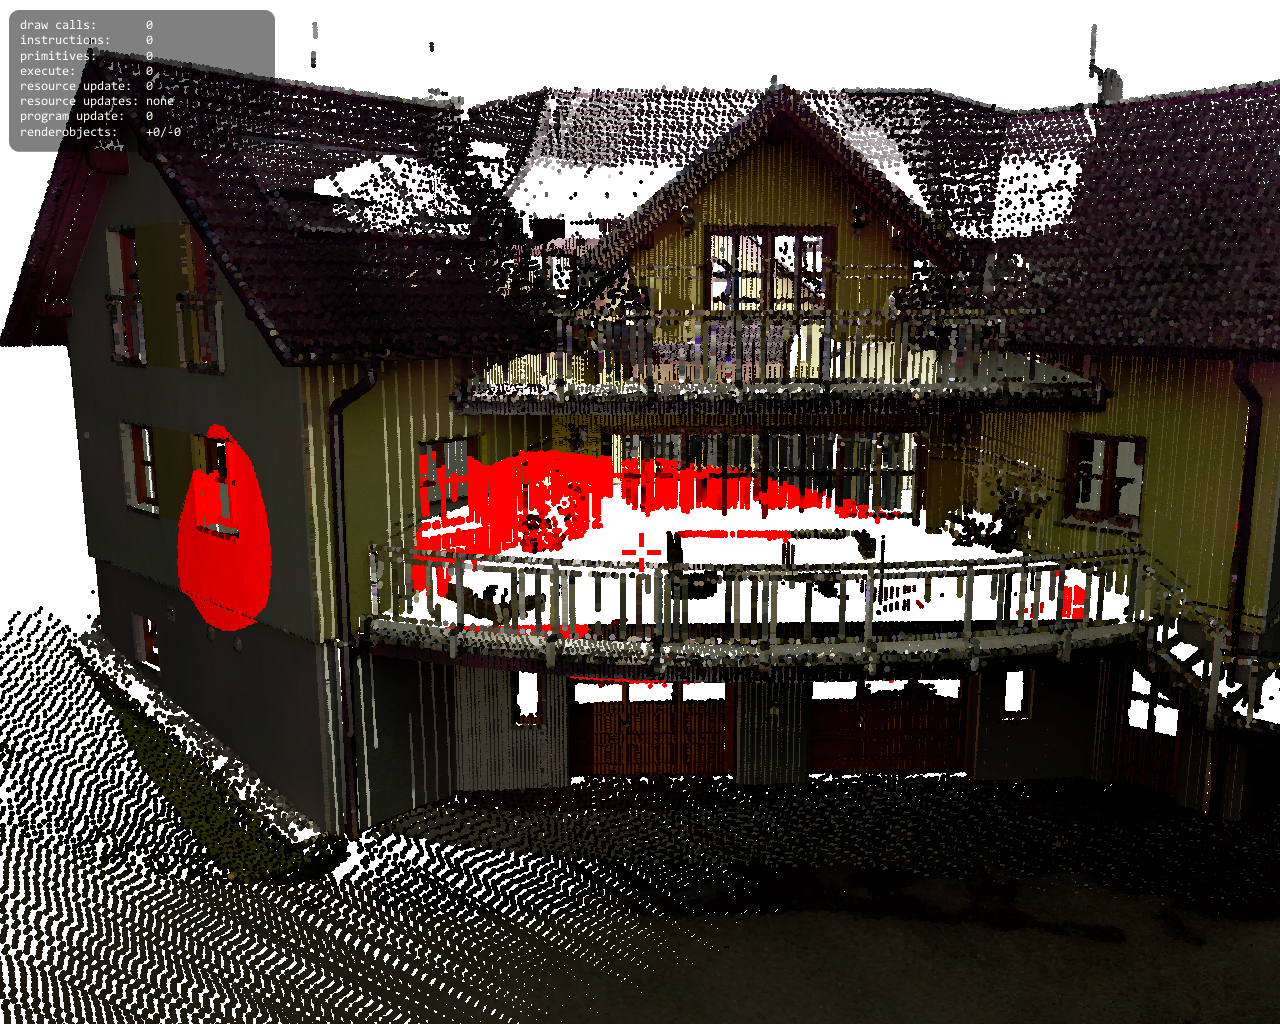
\includegraphics[width=0.5\textwidth]{Interactions/lasso3.png}%
  }
	
\caption{(a) - (c) show a lasso selection performed on a point cloud. In (a) the user draws a polygon onto the screen. In (b) the selected points are visualized in red. Figure (c) showcases the selection from a different angle. All points that are projected to the area of the polygon, are selected. This results in the unintentional selection of points that are obscured by objects in the foreground.}
\label{fig:lasso}
\end{figure}


Figure \ref{fig:lasso} shows a lasso selection performed on a point cloud. The user draws a polygon onto the screen. The selected points are highlighted in red. When changing the view, selected points that where occluded when drawing the lasso, appear. The user must control the selection distance by hand in order to minimize this effect. However, the in order to solve the task of only selecting points on the wall, further lasso selections must be used to remove points from the selection that where selected unintentionally. 





\subsection{Shape-Assisted Region Selection}
\section{Shape-Assisted Local Level-of-Detail Increase}




\backmatter

% Use an optional list of figures.
\listoffigures % Starred version, i.e., \listoffigures*, removes the toc entry.

% Use an optional list of tables.
\cleardoublepage % Start list of tables on the next empty right hand page.
\listoftables % Starred version, i.e., \listoftables*, removes the toc entry.

% Use an optional list of alogrithms.
\listofalgorithms
\addcontentsline{toc}{chapter}{List of Algorithms}

% Add an index.
\printindex

% Add a glossary.
\printglossaries

% Add a bibliography.
\bibliographystyle{alpha}
\bibliography{intro}

\end{document}